\documentclass[12pt]{article}
\usepackage[utf8]{inputenc}
\usepackage[english]{babel}
\usepackage[natbibapa]{apacite} % Stick with apacite for APA style
\usepackage{amsmath}
\usepackage{amssymb}
\usepackage{float}
\usepackage[outputdir=../]{minted}
\usepackage{framed}
\usepackage{lscape}
\usepackage{derivative}
\usepackage{rotating}
\usepackage{placeins}
\usepackage{booktabs}
\usepackage[hmargin=0.7in,vmargin=1in]{geometry}
\usepackage[dvipsnames]{xcolor}
\usepackage{setspace}
\usepackage{bbold}
\usepackage{pdfpages}
\usepackage{longtable}
\usepackage{adjustbox}
\usepackage{caption}
\usepackage[flushleft]{threeparttable}
\usepackage{multirow}
\usepackage{pdflscape}
\usepackage{tikz}
\usetikzlibrary{shapes,arrows}
\usepackage{subcaption} 
\usepackage{hyperref}

\hypersetup{
    unicode=true,
    pdftoolbar=true,
    pdfmenubar=true,
    pdffitwindow=false,
    pdfstartview={FitH},
    pdftitle={Working Draft Latam Paper},
    pdfauthor={}, 
    pdfsubject={},
    pdfcreator={},
    pdfkeywords={},
    pdfnewwindow=true,
    colorlinks=true,
    linkcolor=blue,
    citecolor=blue,
    filecolor=black,
    urlcolor=black
}

\def\qed{\rule{2mm}{2mm}}

\parskip = 1.5ex plus 0.5 ex minus0.2 ex

\newtheorem{theorem}{Theorem}[section]
\newtheorem{lemma}{Lemma}[section]
\newtheorem{definition}{Definition}[section]
\newtheorem{example}{Example}[section]
\newtheorem{corollary}{Corollary}[section]
\newtheorem{remark}{Remark}[section]
\newtheorem{assumption}{Assumption}[section]
\newtheorem{algorithm}{Algorithm}[section]
\setlength\parindent{0pt}

\newcommand*{\h}{\hspace{5pt}}% for indentation
\newcommand*{\hh}{\h\h}% double indentation





 


 \title{ Gender Composition in Classrooms: Influences on Post-Secondary Schooling  Choices \thanks{I thank ....
} }

 
\author{
{ 
\href{https://polanco-jaime.github.io/}{Jaime Polanco-Jiménez}\thanks{Corresponding author, PhD Student at KU Leuven \& Pontificia Universidad Javeriana.    (email:
\href{mailto:jaime.polanco@javeriana.edu.co}{jaime.polanco@javeriana.edu.co} ) %, Tel: +57 3002737490.
  }   
 }\\
  {
Kristof De Witte \thanks{ KU Leuven \& UNU-Merit, Maastricht University.  (email: \href{mailto:: kristof.dewitte@kuleuven.be}{ kristof.dewitte@kuleuven.be}).  } 
 }
 \\
  {
Gloria L. Bernal \thanks{  Pontificia Universidad Javeriana.  (email: \href{mailto:: gbernal@javeriana.edu.co}{ gbernal@javeriana.edu.co}).  } 
 }   
}

 
 \date{\normalsize\today} 
% \singlespacing
\doublespacing 
% \onehalfspacing

\begin{document}
\renewcommand{\BOthers}[1]{et al.\hbox{}}
\maketitle

\abstract{ 
\singlespacing 
% \onehalfspacing
\noindent   
 
This study explores the impact of male students' presence in classrooms on the choice of university majors among female students. To unpack this, we employ a fixed-effects methodology and a staggered difference-in-difference (S-DiD) approach, specifically examining gender compositions within classrooms concerning university major choices.Our findings reveal that, compared to their male counterparts, female students show a significantly higher inclination toward pursuing academic majors associated with human sciences. These results suggest that classrooms with a high composition of male students narrow the gap in STEM majors for women, except in fields such as Law and Medicine. Furthermore, no gender differences were found based on classroom gender composition in majors related to agriculture, zootechnics, and veterinary sciences.


\vspace*{0.3cm}
\textit{JEL} Codes:   O28, I21.\\ %, L71, C93, C21.
\vspace*{0.1cm}
% \vspace*{0.3cm} 
\textbf{Keywords: } 
\\
}

\vfill

%---------------------------------------------------------------------------------------
\newpage    

         
 

%%%%%%%%%%%%%%%%%%%%%%%%%%%%%%%%%%
\section{Introduction}\label{section:01}
 

% \section{Introduction}\label{section:01}

% The underrepresentation of women in science, technology, engineering, and mathematics (STEM) fields is a persistent global challenge. Studies consistently highlight the substantial income advantage associated with STEM careers, making these fields highly desirable. For instance, \citet{nsf2023} reports a 35\% income advantage for STEM careers in 2023. However, despite these incentives, women remain less likely than men to pursue STEM education and careers. This disparity limits women's economic opportunities and deprives STEM fields of valuable talent. This paper examines whether the gender composition of classrooms influences female students' choices of university majors, particularly in STEM fields. 

% We focus on the case of Colombia, where a significant gender gap persists in STEM fields despite women achieving higher overall university graduation rates. Data from the Instituto Colombiano para la Evaluación de la Educación \citep{ICFES2019} reveals that only 16\% of female university graduates choose STEM careers, compared to 24\% of male graduates. 

% This study investigates the hypothesis that the presence of male students, often exhibiting higher levels of competitiveness, influences female students' career aspirations. Research shows that women often respond less favorably to competition than men, especially in mixed-gender environments \citep{Niederle2011}.  For example, \citet{Gindi2019} found that while girls demonstrate greater competitiveness in verbal tasks, boys tend to be more competitive in motor and spatial domains. Moreover, \citet{Thomas2014} established a link between competitiveness and career preferences, demonstrating that highly competitive individuals (often male) are more likely to pursue STEM-related disciplines. This suggests that classroom gender composition may affect female students' competitiveness and, consequently, their choice of university majors. A higher proportion of male students could foster a more competitive environment, potentially nudging female students towards STEM fields and deterring them from humanities-related disciplines.

% To test this hypothesis, we analyze a comprehensive dataset encompassing the Integrated School Enrollment System in Colombia \citep{SIMAT}, the National Higher Education Information System \citep{SNIES}, and the Formal Education Survey \citep{EDUC}.  Our empirical strategy employs both fixed-effects models and a staggered difference-in-differences (S-DiD) design. Fixed-effects models allow us to control for unobserved student and school characteristics that might influence both classroom gender composition and major choices. Additionally, the S-DiD approach exploits the natural experiment of schools transitioning from single-sex to co-educational settings, allowing us to estimate the causal impact of changing gender composition on female students' university major choices.

% Our findings reveal that classroom gender composition does indeed influence female students' major choices. We find that a higher proportion of male students in a classroom is associated with a decreased likelihood of female students opting for STEM-related careers.  This suggests that increased male presence might not necessarily encourage female students into STEM fields, as hypothesized. Additionally, we observe varying effects across different academic disciplines, with female students exhibiting a higher preference for traditionally female-dominated fields like social sciences and humanities in classrooms with greater male representation. These findings underscore the complex interplay of gender dynamics, competitiveness, and societal expectations in shaping educational choices.


% This research makes three important contributions. Firstly, it provides the first empirical investigation of the relationship between classroom gender composition and female students' university major choices in Colombia, a developing country with a persistent gender gap in STEM fields \citep{informe2023lee}. While existing research often explores peer gender effects on major choice within specific contexts, such as business schools \citep{zolitz2021effect}, this study examines a broader range of academic disciplines.  Moreover, it moves beyond examining the influence of gender composition on academic performance \citep{EISENKOPF2015123, Pregaldini2020} to explicitly focus on its impact on major selection, providing valuable insights into the mechanisms shaping career aspirations. Secondly, this research examines the nuanced effects of varying gender compositions within mixed-gender classrooms.  This contrasts with studies that examine broader differences between single-sex and co-educational settings \citep{bernal2022effect}, offering a more fine-grained understanding of how classroom gender dynamics affect female students' post-secondary decisions. Finally, this study has important implications for policymakers and educators in Colombia, and potentially other developing countries, seeking to promote gender equality in STEM fields. By understanding the dynamics of gender composition in classrooms, interventions can be tailored to create more inclusive learning environments that foster a more equitable distribution of talent across diverse academic disciplines.

The underrepresentation of women in science, technology, engineering, and mathematics (STEM) fields is a persistent global challenge. Studies consistently highlight the substantial income advantage associated with STEM careers, making these fields highly desirable. For instance, \citet{nsf2023} reports a 35\% income advantage for STEM careers in 2023. However, despite these incentives, women remain less likely than men to pursue STEM education and careers. This disparity limits women's economic opportunities and deprives STEM fields of valuable talent. This paper examines whether the gender composition of classrooms influences female students' choices of university majors, particularly in STEM fields. 

We focus on the case of Colombia, where a significant gender gap persists in STEM fields despite women achieving higher overall university graduation rates. Data from the Instituto Colombiano para la Evaluación de la Educación \citep{ICFES2019} reveals that only 16\% of female university graduates choose STEM careers, compared to 24\% of male graduates. 

This study investigates the hypothesis that the presence of male students, often exhibiting higher levels of competitiveness, influences female students' career aspirations. Research shows that women often respond less favorably to competition than men, especially in mixed-gender environments \citep{Niederle2011}.  For example, \citet{Gindi2019} found that while girls demonstrate greater competitiveness in verbal tasks, boys tend to be more competitive in motor and spatial domains. Moreover, \citet{Thomas2014} established a link between competitiveness and career preferences, demonstrating that highly competitive individuals (often male) are more likely to pursue STEM-related disciplines. This suggests that classroom gender composition may affect female students' competitiveness and, consequently, their choice of university majors. A higher proportion of male students could foster a more competitive environment, potentially nudging female students towards STEM fields and deterring them from humanities-related disciplines.

To test this hypothesis, we analyze a comprehensive dataset encompassing the Integrated School Enrollment System in Colombia \citep{SIMAT}, the National Higher Education Information System \citep{SNIES}, and the Formal Education Survey \citep{EDUC}.  Our empirical strategy employs both fixed-effects models and a staggered difference-in-differences (S-DiD) design. Fixed-effects models allow us to control for unobserved student and school characteristics that might influence both classroom gender composition and major choices. Additionally, the S-DiD approach exploits the natural experiment of schools transitioning from single-sex to co-educational settings, allowing us to estimate the causal impact of changing gender composition on female students' university major choices.

Our findings reveal that classroom gender composition does indeed influence female students' major choices. We find that a higher proportion of male students in a classroom is associated with a decreased likelihood of female students opting for STEM-related careers \textcolor{red}{[value]}.  This suggests that increased male presence might not necessarily encourage female students into STEM fields, as hypothesized. Additionally, we observe varying effects across different academic disciplines, with female students exhibiting a higher preference for traditionally female-dominated fields like social sciences and humanities in classrooms with greater male representation \textcolor{red}{[value]}. These findings underscore the complex interplay of gender dynamics, competitiveness, and societal expectations in shaping educational choices.

This research makes three important contributions. Firstly, it provides the first empirical investigation of the relationship between classroom gender composition and female students' university major choices in Colombia, a developing country with a persistent gender gap in STEM fields \citep{informe2023lee}. While existing research often explores peer gender effects on major choice within specific contexts, such as business schools \citep{zolitz2021effect}, this study examines a broader range of academic disciplines.  Moreover, it moves beyond examining the influence of gender composition on academic performance \citep{EISENKOPF2015123, Pregaldini2020_1} to explicitly focus on its impact on major selection, providing valuable insights into the mechanisms shaping career aspirations. Secondly, this research examines the nuanced effects of varying gender compositions within mixed-gender classrooms.  This contrasts with studies that examine broader differences between single-sex and co-educational settings \citep{bernal2022effect}, offering a more fine-grained understanding of how classroom gender dynamics affect female students' post-secondary decisions. Finally, this study has important implications for policymakers and educators in Colombia, and potentially other developing countries, seeking to promote gender equality in STEM fields. By understanding the dynamics of gender composition in classrooms, interventions can be tailored to create more inclusive learning environments that foster a more equitable distribution of talent across diverse academic disciplines.


The remainder of this article is organized as follows. Section \ref{section:02} presents the data used in this study. The empirical strategy, including the mechanism by which gender composition can affect post-secondary study choices, is presented in Section \ref{section:03}. The results are discussed in Section \ref{section:04}, and the article concludes in Section \ref{section:05}. Robustness checks and additional results are reported in the Appendix. 

% The underrepresentation of women in science, technology, engineering, and mathematics (STEM) fields is a persistent global challenge.  Studies consistently highlight the substantial income advantage associated with careers in STEM compared to other fields. For instance, The \citet{nsf2023} reports a 35\% income advantage for STEM careers, emphasizing the significant financial incentives driving educational choices. Despite this, women remain less likely than men to pursue these fields.  This disparity limits women's economic opportunities and deprives STEM fields of valuable talent. This paper examines whether the gender composition of classrooms influences female students' choices of university majors, particularly in STEM fields. 


% We focus on the case of Colombia, where a significant gender gap in STEM fields persists despite women achieving higher overall university graduation rates. Data from the Instituto Colombiano para la Evaluación de la Educación \citep{ICFES2019} reveals that only 16\% of female university graduates choose STEM careers, compared to 24\% of male graduates.  

% This study explores the hypothesis that the presence of male students, often exhibiting higher levels of competitiveness, exerts a distinct influence on female students' career aspirations and decisions.  Research has shown that women often respond less favorably to competition than men, particularly in mixed-gender environments \citep{Niederle2011}.  \citet{Gindi2019} found that while girls demonstrated greater competitiveness in verbal tasks, boys tended to be more competitive in motor and spatial domains.   Furthermore, \citet{Thomas2014} established a link between competitiveness and career preferences, showing that highly competitive individuals, often male, are more likely to pursue STEM-related disciplines. This suggests that the gender composition of classrooms may influence female students' competitiveness and, consequently, their choice of university majors.  A higher proportion of male students in a classroom could foster a more competitive environment, potentially nudging female students towards STEM fields while deterring them from humanities-related disciplines. 
 
% To test these hypotheses, we analyze a comprehensive dataset encompassing the Integrated School Enrollment System in Colombia \citep{SIMAT}, the National Higher Education Information System \citep{SNIES}, and the Formal Education Survey \citep{EDUC}.  Our empirical strategy leverages both fixed-effects models and a staggered difference-in-differences (S-DiD) design.  The fixed-effects models allow us to control for unobserved student and school characteristics that might influence both classroom gender composition and major choices. We use the S-DiD approach to exploit the natural experiment of schools transitioning from single-sex to co-educational settings, providing a causal estimate of the impact of changing gender composition on female students' university major decisions.



% This research makes three important contributions to the understanding of gender dynamics and educational choices. First, it provides the first empirical investigation of the relationship between classroom gender composition and female students' university major choices in Colombia, a developing country with a persistent gender gap in STEM fields\citep{informe2023lee}. While existing research often explores the effects of peer gender on major choice within specific contexts, such as business schools \citep{zolitz2021effect}, this study takes a broader approach, examining a wider range of academic disciplines.  Additionally, while existing research highlights the influence of gender composition on academic performance \citep{EISENKOPF2015123, Pregaldini2020}, this study explicitly examines its impact on major selection, offering insights into the mechanisms driving career aspirations. Second, this research delves deeper into the impact of varying gender compositions within mixed-gender classrooms. In contrast to studies that focus on the broader differences between single-sex and co-educational settings \citep{bernal2022effect}, this study examines the nuanced effects of different male-to-female ratios within mixed-gender classrooms. This approach provides a more fine-grained understanding of how gender dynamics within the classroom influence female students' post-secondary schooling decisions. Finally, our findings have important implications for policymakers and educators in Colombia and potentially other developing countries seeking to promote gender equality in STEM fields. By understanding the dynamics of gender composition in classrooms, interventions can be tailored to create more inclusive learning environments that foster a more equitable distribution of talent across diverse academic disciplines.


% The remainder of this article is organized as follows. Section \ref{section:02} presents the data used in this study. The empirical strategy, which allows for the estimation of causal inference, including the mechanism by which gender composition can affect post-secondary study choices, is presented in Section \ref{section:03}. The results are discussed in Section \ref{section:04}, and the article concludes in Section \ref{section:05}.  Robustness checks and additional results are reported in the Appendix. 


 
%%%%%%%%%%%%%%%%%%%%%%%%%%%%%%%%%%
% \section{Context and Background}
\section{Data and Descriptive Statistics}\label{section:02}
In our empirical investigation into the intricate relationship between gender, school composition, and post-secondary study decisions, we leverage comprehensive datasets from three primary sources: the Integrated School Enrollment System in Colombia (SIMAT), the National Higher Education Information System (SNIES), and the Formal Education Survey (EDUC).

The Integrated School Enrollment System in Colombia (SIMAT) serves as a fundamental resource in our research, providing detailed records of student enrollment and academic progress throughout their educational journey. This system offers a longitudinal perspective, enabling us to track individuals over time and analyze trends in educational outcomes.

Similarly, the National Higher Education Information System (SNIES) offers invaluable insights into post-secondary education in Colombia. With its extensive database of higher education institutions, programs, and student enrollment data, SNIES allows us to explore the majors students choose after completing secondary school. By examining enrollment patterns and graduation rates, we can better understand the dynamics of post-secondary education and its implications for future career paths.

To complement our analysis of individual-level data, we turn to the Formal Education Survey (EDUC), which provides detailed information about school attributes and educational environments. By examining factors such as school size, resources, and student demographics, we gain a more holistic understanding of the contextual nuances shaping the relationship between gender, school composition, and post-secondary study decisions.


In table \ref{tab:gender_dist2}, we present the distribution of students across different gender compositions in secondary schools. This table illustrates the proportion of male students in each school, ranging from 0 (representing single-gender female schools) to 1 (representing single-gender male schools). It is important to note that the values at the extremes (0 and 1) denote single-gender schools, which are excluded from the descriptive analysis. These single-gender schools lack sample variation within the school, thereby limiting their utility when calculating the relationship between studying a major and gender as a conditioning factor.

\begin{table}[!htbp] 
    \centering
    \begin{tabular}{cccccc}
    \hline \hline 
         Min. & 1st Qu. & Median  &  Mean & 3rd Qu.  &  Max.          \\\hline  \hline 
         0.000 &  0.377 & 0.462 & 0.457 & 0.546 &  1.000         \\
    \hline
    \end{tabular}
\caption{Proportion of Male Students in the Last Year of Secondary Schools}
\label{tab:gender_dist2}
\end{table}


 
 
From Figure \ref{histograma_male_fraction}, we observe a typical distribution representing the gender composition within classrooms, revealing an approximate mean with 46\% women. In it, we identify two main challenges. Firstly, single-gender schools transitioning to mixed schools encounter what we term 'corner decisions.' Secondly, students attending mixed schools, where classrooms have varying gender compositions, alter their post-secondary career choices due to gender reinforcement dynamics within the classroom.


\begin{figure}[H] % Use [h] to try to place the figure "here"
    \centering
    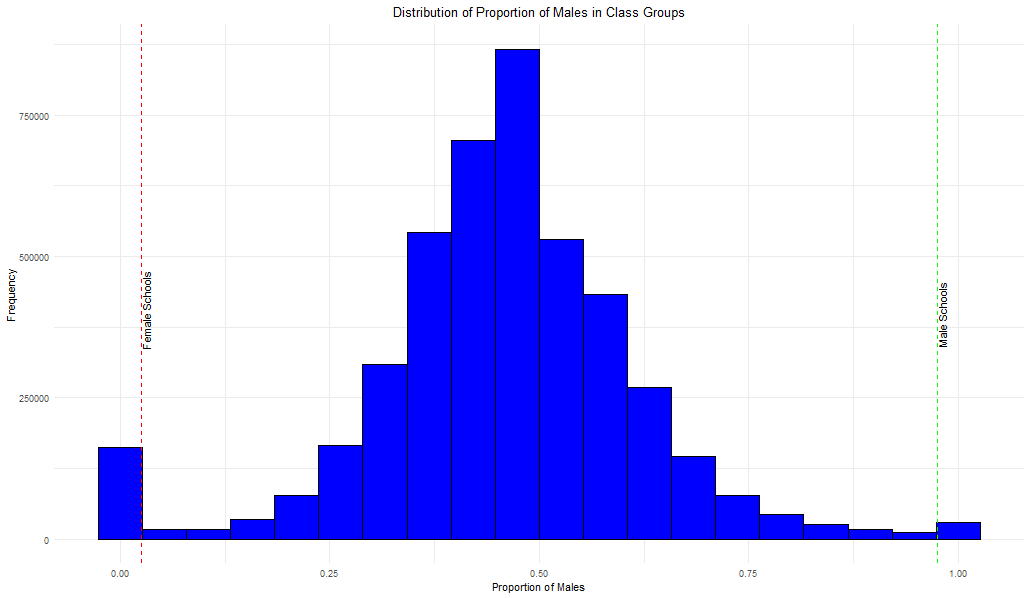
\includegraphics[width=0.7\linewidth]{Graph/his_frac_males.png} % Adjust width as needed
    \caption{Distribution of Proportion of Males in Class Groups}
    \label{histograma_male_fraction}
\end{figure}


%%%%%%%%%%%%%%%%%%%%%%%%%%%%%%%%%%


%%%%%%%%%%%%%%%%%%%%%%%%%%%%%%%%%%
\section{ Empirical Strategy}\label{section:03}


This study delves into the influence exerted by the gender composition within secondary schools on students' decisions regarding their choice of university majors. To achieve this, we undertake an examination of participation rates across ten distinct fields of study , each representing potential post-secondary career paths. Our investigation employs two distinct methodologies to ensure comprehensive analysis, while also exploring the underlying mechanisms driving these relationships.


\subsection{Mechanism}
The accumulation of human capital and post-secondary school decisions, particularly in the selection of a major university, is discussed in studies such as \citet{Hanushek1979} and \citet{Petra2003}. In these studies, the decision results from a multifaceted interaction between expected future income, budget constraints when the student makes the decision, family attributes, student attributes, school attributes, and social influences to which students are exposed. Among these factors, student attributes play a critical role, encompassing intelligence, motivation, study habits, competitiveness, and other influential characteristics \footnote{Studies by \citet{LONNQVIST2015254} and \citet{Thomas2014} demonstrate the impact of risk attitudes and self-confidence on students' academic choices.}.

\citet{NBERw22010} explicates the life cycle of households in three distinct stages: education, early work, and late work. This progression is supported by theoretical models of human capital accumulation (refer, for instance, to \citet{BenPorath}). Theoretical models of human capital accumulation predominantly hinge on the time available for students to dedicate to their studies. Having more time to study directly correlates with spending less time on early work. However, this also implies a budgetary constraint when deciding whether to pursue further studies and which field to study.  

Environmental factors, including social support and media, significantly influence students' interest in STEM careers, as revealed by \citet{Wang2023Gender}. The study highlights that male students generally exhibit higher interest in STEM careers compared to female students. The influence mechanisms differ, with social support being more impactful for males and media playing a greater role for females. 
 
Another perspective on gender roles is provided by \citet{Alesina2013}, who explore the historical origins of cross-cultural differences in beliefs and values regarding the appropriate role of women in society. The study focuses on the influence of traditional agricultural practices, particularly plough agriculture, on the evolution of gender norms. The findings suggest that societies with a heritage of traditional plough use exhibit less equal gender norms in contemporary beliefs and practices, even among the descendants living in diverse environments. This underlines the lasting impact of historical practices on contemporary societal values and gender roles.

According to the OECD (\citet{pisa_mechanism}), motivated students achieve better performance in mathematics, and in this sense mathematics performance in school is a predictor of choosing a STEM major at university (\citet{Kohen2022}).
 

The investigation conducted by \citet{Sutter2010gender} revealed a notable gender-based divergence in competitiveness, wherein males exhibited a heightened level by 15 to 20 percentage points compared to the average competitiveness observed in females. This discernible gap in competitiveness is particularly intriguing as it manifests as early as 4 to 5 years of age, underscoring the early emergence of gender disparities in this trait. Additionally, \citet{Gindi2019} extended these findings by highlighting that boys tend to manifest greater competitiveness in motor and spatial domains, while girls demonstrate heightened competitiveness in verbal areas.

Furthermore, empirical support for the association between the desire for competitiveness and career choices is provided by \citet{Thomas2014}. This experimental study establishes a robust connection between individuals' inclination toward competitiveness and their career preferences. Notably, the findings of this study suggest that men tend to display a greater proclivity for competitiveness compared to women. Moreover, it underscores a direct correlation between the level of competitiveness and the chosen academic major at the university level. Intriguingly, highly competitive individuals predominantly opt for disciplines within the Science, Technology, Engineering, and Mathematics (STEM) domain.



\begin{center}
    \begin{tabular}{lllll}
        \begin{tabular}[c]{@{}l@{}}Proportion of male \\ students in a classroom\end{tabular} & $\Rightarrow$ & \begin{tabular}[c]{@{}l@{}}Female\\ competitiveness\end{tabular} & $\Rightarrow$ & \begin{tabular}[c]{@{}l@{}}University \\ major choice\end{tabular}
    \end{tabular}
\end{center}

Therefore, it is anticipated that the gender composition within a classroom significantly influences female competitiveness. A higher proportion of male students may suggest a narrowing gender gap in career selection, primarily attributed to the impact of competitiveness emanating from male peers. This influence could exhibit variations across academic domains, with fields associated with humanities, social sciences, economics, and languages—traditionally dominated by female students—experiencing a decline in female participation relative to male involvement when influenced by their male counterparts.

In contrast, within STEM-related disciplines, it is expected that female students will demonstrate a reduction in the gender gap, driven by the substantial influence exerted by male peers in the classroom. Essentially, the presence of male students alters the behavioral dynamics of female students, leading to a diminished participation gap between men and women.

 

An additional interpretation regarding marginal effects and the significance of these coefficients could enhance the understanding of how the likelihood of choosing a specific major changes with varying gender compositions in secondary schools. For example, a positive \(\beta_1\) might suggest a certain increase in the probability of a female student choosing the specified major compared to male students, specifically considering a change in the gender composition of their class.
%%%%%%%%%%%%%%%%%%%%%%%

Moreover, the incorporation of school-fixed effects enables the consideration of inherent and stable characteristics unique to different educational institutions.
School-fixed effects allow us to account for the intrinsic and stable characteristics of different schools. For instance, some schools may emphasize technology, business, or industry-related subjects. The geographical features and physical attributes of a school may remain consistent and unique across different generations. It includes the socio-demographic and economic conditions of the students in a school that remain constant.

Furthermore, time-fixed effects help to capture systematic variations that occur over time. Changes in societal norms, economic conditions, and government policies, as well as other temporal trends, can influence educational choices over different periods. These time-specific effects are crucial for a more comprehensive understanding of the changing landscape of educational decisions made by individuals, particularly women entering university programs.


\subsection{Methodology 1: Event-Study Regressions}

To address potential biases intrinsic to fixed effect estimation, we employ a distinct approach by leveraging the transition from single-sex schools to co-educational settings. This unanticipated shift serves as an intervention influencing student behavior, enabling a more robust examination of its effects.

Our study encompasses all public schools in Colombia that have undergone this transition, allowing us to track student enrollments across diverse academic fields at the university level. Employing a Staggered Difference-in-Differences design (S-DiD), we compare schools that have undergone the transition with those that, as of 2020, had not yet experienced the shift (treated schools versus no treated yet schools). This methodological strategy helps reveal the causal impact of the transition on student choice at university, offering insight into the implications arising from the change in school structure on students' university enrollment patterns.

\begin{equation} 
\hat{\tau} = \bar{Participation^P_{ \text{after transition}} } - \bar{Participation^P_{ \text{before transition}} }
\end{equation}

Where \( \hat{\tau} \) represents the change in the average participation of students in the academic major \( P \) before and after the transition from single-sex to co-educational schooling.

Given your focus on the participation of students in major \( P \) before and after a transition, the adapted formula might look something like this (based on \citet{SUN2021175} ):

\begin{equation} 
\text{Participation}_{c,t,j}^P = \beta_0 + \sum_{\varphi = -S}^{-2} \mu_{\varphi} \cdot D_{c,\varphi} + \sum_{\varphi = 0}^{M} \mu_{\varphi} \cdot D_{c,\varphi} + \sigma_t + \gamma_c + \varepsilon_{c,t}
\end{equation}

Here:
- \( \text{Participation}_{c,t,j}^P \) represents the level of participation of students in major \( P \) at a particular school \( c \) and time \( t \).
- \( \beta_0 \) is the intercept or baseline level of participation in major \( P \).
- \( \mu_{\varphi} \) are the parameters associated with the different time periods or treatment phases \( \varphi \).
- \( D_{c,\varphi} \) are dummy variables denoting the treatment status (e.g., before and after the transition) for school \( c \) at time \( \varphi \).
- \( \sigma_t \) captures time-specific effects.
- \( \gamma_c \) captures school-specific effects.
- \( \varepsilon_{c,t} \) is the error term.

By including both time-specific and school-specific effects in the estimation, the analysis can better account for and control various unobserved factors that might influence students' choices of university majors. This helps provide a more accurate understanding of the specific influence of transitioning from single-sex to co-educational schooling on the participation of students in the specified academic major, resulting in more robust and reliable estimations.

The time-specific fixed effect is crucial as it captures broader trends or fluctuations that might affect student participation in academic majors, regardless of the transition being studied. Societal changes, economic shifts, or educational reforms occurring independently of the transition could impact students' major choices. By including these effects, the model more effectively isolates the transition's specific impact on student decisions.

Conversely, the school-specific fixed effect addresses persistent differences between schools, unrelated to the transition itself. Each school possesses unique attributes, teaching methods, or cultural distinctions that could influence students' major choices. Incorporating these school-specific effects helps the model accommodate these differences, effectively separating the transition's impact from inherent school-specific variations.

To address potential biases intrinsic to fixed effect estimation, our approach hinges on leveraging the transition from single-sex schools to coeducational settings as a natural intervention influencing student behavior. This unanticipated shift provides a unique opportunity for a robust examination of its effects.

\vspace{5mm}
\textit{Identification Strategy}
\vspace{3mm}

Our study aims to ascertain the causal effect of Colombian schools transitioning from single-sex to coeducational settings on students' choice of university majors post-graduation. This is accomplished through the utilization of a staggered difference-in-differences (S-DiD) design, which involves a comparison between schools that have already undergone the transition and those that have not yet done so as of 2020.

The effectiveness of the S-DiD design relies on several critical assumptions. Firstly, we assume parallel trends in the absence of the transition, implying that the trends in students' choice of major P would have evolved similarly between schools that transitioned and those that have not yet transitioned, under the influence of common unobserved factors affecting major choice across schools.

Additionally, we assume the absence of concurrent shocks differentially affecting treated and untreated schools over the study period, apart from the transition itself. The inclusion of time fixed effects helps in adjusting for broader secular trends. Furthermore, we assume no anticipation of the transition's impact on student behavior until its actual occurrence, and test for any anticipatory effects by examining leads of the treatment indicator.

Moreover, the irreversibility assumption posits that once a school transitions, it remains coeducational throughout the study period, with no schools reverting to single-sex education within the sample. We also rely on the presence of overlapping cohorts within each school at any given time, enabling the observation of treated and untreated cohorts concurrently to identify the effect.

Finally, we assume the stability of student and school compositions over time. School fixed effects are incorporated to adjust for time-invariant compositional differences across schools.

The staggered timing of schools' transitions provides variation in treatment status over time. By comparing outcomes between treated and untreated schools before and after the transitions, and conditioning on school and time fixed effects, we can effectively isolate the causal effect of the transition, contingent upon the validity of the aforementioned assumptions.

\subsection{Methodology 2: Probability Estimation based on Gender Composition}

In this secondary analysis, we compute the probability that a secondary school student, denoted as $i$, selects a particular university major $c$ based on the gender composition within their classroom. For instance, a gender composition of 0.2 signifies that a secondary female student, denoted as $i$, studied in a classroom where 20\% of the students were male, while the remaining 80\% were female.

To gauge the likelihood of a secondary school student opting for a specific university major contingent upon the classroom gender composition, we segment the groups based on specific proportions of male students within each classroom.

Moreover, as an integral part of our analytical framework, we have adapted the methodology proposed by \citet{IMBENS2012}. This methodology, focusing on minimizing the mean squared error to identify similar groups based on their outcome variable, has been tailored to segment a range of fractions of male students in a classroom who make similar study decisions. This adaptation is founded on the Binary Cross Entropy loss function (\citet{Mao2023}), with a detailed explanation provided in Appendix \ref{bce}.

This estimate pertains to each student represented as $i$. Therefore, the relationship is expressed as follows:

\begin{equation}
     \log\left(\frac{P(Y_{i,s,t}^c  = 1)}{1 - P(Y_{i,s,t}^c  = 1)}\right) =  
       \beta_1 \times Gender_{i,s,t} +
       \beta_2 \times X_{i,s,t}^c  + \gamma_{t} + \gamma_{s} + 
       \varepsilon_{i,s,t}
\end{equation}

Where $Y_{i,s,t}^c$ is the binary response variable for students $i$ who have completed secondary school in the school $s$. It takes the value of 1 when a student $i$ chooses a university major $c$ and 0 otherwise. $Gender_{i,s,t}$ takes the value of 1 for female students of a secondary school. $X_i$ is a vector of student $i$ characteristics in each secondary school. The model includes school fixed effects ($\gamma_{t} $), year fixed effects ($\gamma_{t}$), and the usual error term $\varepsilon_{i,s,t}$.

$\beta_1$ is the coefficient of interest that specifically represents the relationship between being a female student (denoted as \( Gender = Female \)) and the log-odds of a female student choosing a particular university major $c$, while holding other variables constant in the model. A positive value for $\beta_1$ suggests a positive correlation between being a female student and the likelihood of choosing the academic major 'c' compared to male students. This means that, all else being equal, being a female student is associated with a higher probability of choosing the specified academic major 'c' as compared to being a male student.

The table  \ref{tab:summary_bce} provides a comprehensive summary of key statistics derived from BCE bootstraping estimation, facilitating inference on the optimal distance concerning the selection of university majors based on gender composition within secondary schools. Each row of the table corresponds to a distinct outcome or university major, while the columns offer insights into the mean Binary Cross Entropy (BCE) score, standard deviation, and optimal distance. This optimal distance serves as a critical parameter in the estimation process across various subsets of gender composition settings.

\begin{table}[H]
\centering
\caption{Summary of Bootstrapped BCE Estimation}
\label{tab:summary_bce}
\begin{tabular}{lccc}
\toprule
Outcome                              & Mean BCE & Standard Deviation & Optimal Distance \\ \hline
& \multicolumn{3}{c}{\textbf{BCE Estimation Results}} \\

\midrule
Law & 0.1189 & 0.0117 & 0.0998 \\
Medicine & 0.1000 & 0.0108 & 0.1109 \\
No Studies & 0.7555 & 0.0062 & 0.0832 \\
Health Sciences & 0.1585 & 0.0309 & 0.1109 \\
Education Sciences & 0.1313 & 0.0184 & 0.1109 \\
Agronomy, Veterinary \& Related & 0.1202 & 0.0117 & 0.1109 \\
Social Sciences \& Humanities & 0.2107 & 0.0262 & 0.1109 \\
Mathematics \& Natural Sciences & 0.0988 & 0.0036 & 0.1109 \\
Fine Arts & 0.1041 & 0.0107 & 0.1109 \\
Engineering, Architecture \& Related & 0.4616 & 0.0884 & 0.1109 \\
Economics \& Business Related & 0.3890 & 0.0538 & 0.0832 \\
\hline
\hline
Fixed Effects & \multicolumn{3}{c}{Not Applicable} \\  
S.E. Clustered by: & \multicolumn{3}{c}{Not Applicable} \\
\bottomrule
\end{tabular}
\begin{threeparttable}
\begin{tablenotes}
\small
\item \textbf{Note:} This table presents the results of bootstrapped BCE estimation for different university major categories. The Mean BCE represents the average predictive accuracy of the model, with lower values indicating better performance. The Standard Deviation reflects the variability in BCE scores. The Optimal Distance represents the threshold of gender composition (proportion of male students) in classrooms that minimizes entropy in schooling decisions for each major category.
\item Significance codes: 0 '***' 0.001 '**' 0.01 '*' 0.05 '.' 0.1 ' ' 1
\end{tablenotes}
\end{threeparttable}
\end{table}


The mean BCE score represents the average predictive accuracy of the model in estimating the probability of students choosing a specific major, with lower values indicating better predictive performance. The standard deviation reflects the variability in BCE scores across observations for each major, providing insights into the consistency of model predictions.

Additionally, the optimal distance represents the threshold of gender composition within classrooms that minimizes entropy in schooling decisions for each major. This distance signifies the proportion of male students within a classroom that exerts the most significant influence on students' choices of university majors. For instance, a higher optimal distance suggests that gender composition plays a more substantial role in determining students' decisions regarding that major.

These statistics serve as valuable indicators of the relationship between gender composition and university major selection, shedding light on the nuanced dynamics influencing students' educational trajectories. They provide essential context for understanding the impact of classroom demographics on academic choices and inform policymakers and educators seeking to promote gender diversity and equity within educational settings.


%%%%%%%%%%%%%%%%%%%%%%%%%%%%%%%%%%

%%%%%%%%%%%%%%%%%%%%%%%%%%%%%%%%%%
\section{Results} \label{section:04}

The likelihood of female students selecting specific university majors varies significantly based on the gender composition within their classrooms, as evidenced by the series of figures presented.

\vspace{5mm}
\textit{Female Students Choosing  not to Pursue Further Studies}
\vspace{5mm}

Furthermore, the odds ratio for female students choosing not to pursue further studies also varies with changes in the male composition fraction in the classroom. The overall sample odd ratio for female students not pursuing any further studies is 0.101. However, when the proportion of male students is less than 14\%, the odds ratio decreases to around -0.2. This indicates that the likelihood of female students not continuing their studies increases as the proportion of male students in the classroom increases. This relationship is visually depicted in Figure \ref{fig:no_studies}, illustrating how the likelihood of a female student choosing not to pursue further studies shifts in response to variations in the gender composition of the classroom. 



\begin{figure}[H]
\centering
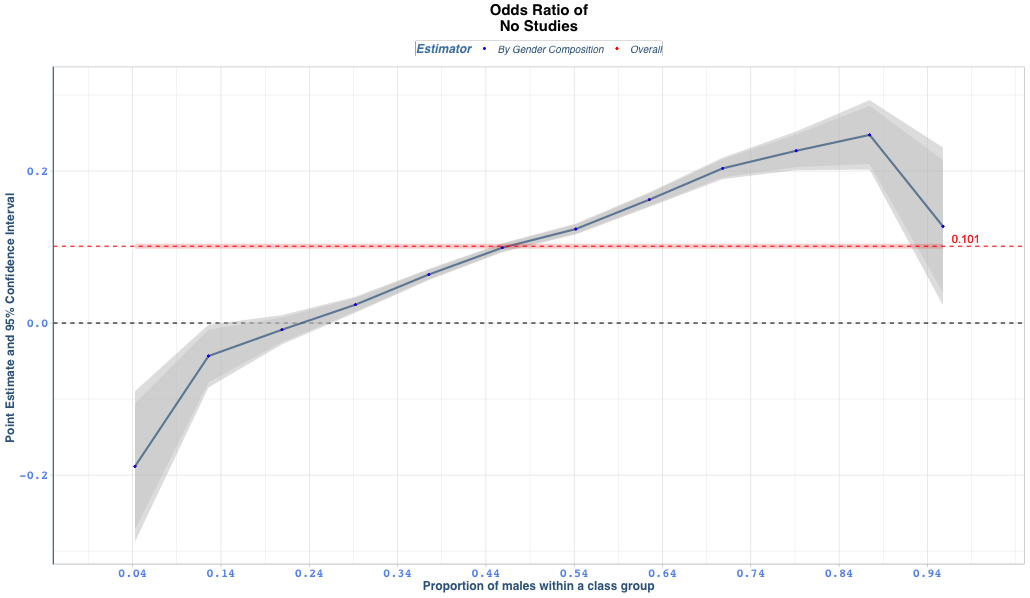
\includegraphics[width=0.8\textwidth]{Graph/Results/fe_panel_student_gender_composition_wome_in_NO_STUDIES_bce.png}
\caption{Likelihood of a female student choosing not to pursue further studies}
\label{fig:no_studies}
\end{figure}
% \subsubsection{Empirical Strategy} \label{empirical_design}

Additionally, when a female school transitions to a coeducational school, the proportion of women who cease studying in the two years following the change tends to increase. This trend is demonstrated in Figure \ref{fig:staggered_females_no_studies}, highlighting the impact of school gender composition changes on female students' study decisions."

\begin{figure}[H]
    \centering
        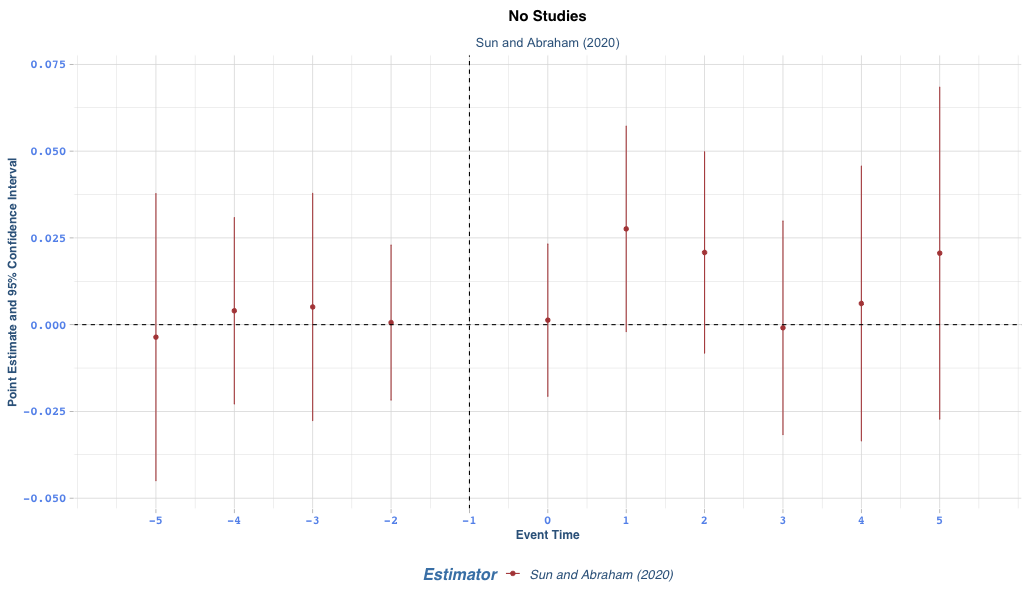
\includegraphics[width=0.8\textwidth]{Graph/Results/stagered_ex_females_NO_STUDIES.png}
        \caption{Proportion of Female Students Not Pursuing Further Studies in Schools Transitioning from Female to Coeducational}
    \label{fig:staggered_females_no_studies}
\end{figure}

\vspace{5mm}
\textit{Female Students Choosing STEM Studies}
\vspace{5mm}


We found that the odds ratio of female students choosing a STEM career reaches 0.92, indicating a significant difference compared to male students in similar classroom compositions. The relationship between classroom gender composition and female students' propensity to pursue STEM studies is depicted in Figure \ref{fig:STEM_studies}, which illustrates how the likelihood of a female student choosing a STEM-related career varies across different proportions of male students in the classroom.

\begin{figure}[H]
\centering
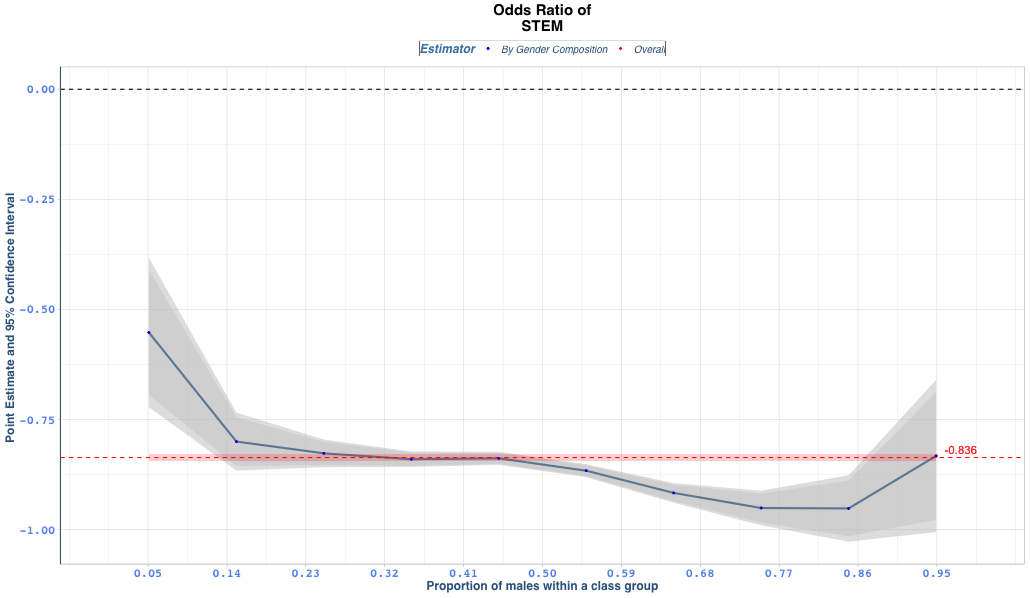
\includegraphics[width=0.8\textwidth]{Graph/Results/fe_panel_student_gender_composition_wome_in_STEM_bce.png}
\caption{Likelihood of a female student choosing a STEM-related career}
\label{fig:STEM_studies}
\end{figure}

When the proportion of male students in the classroom increases, the likelihood of female students opting for STEM-related careers decreases. This finding aligns with existing theories that suggest a correlation between classroom composition, gender dynamics, and career aspirations \citep{Gneezy2003, Thomas2014}. Specifically, in mixed-gender environments, the disparity in competitiveness between men and women tends to widen, with higher levels of competitiveness often associated with a greater inclination towards STEM careers \citep{Thomas2014}.





\begin{figure}[H]
    \centering
        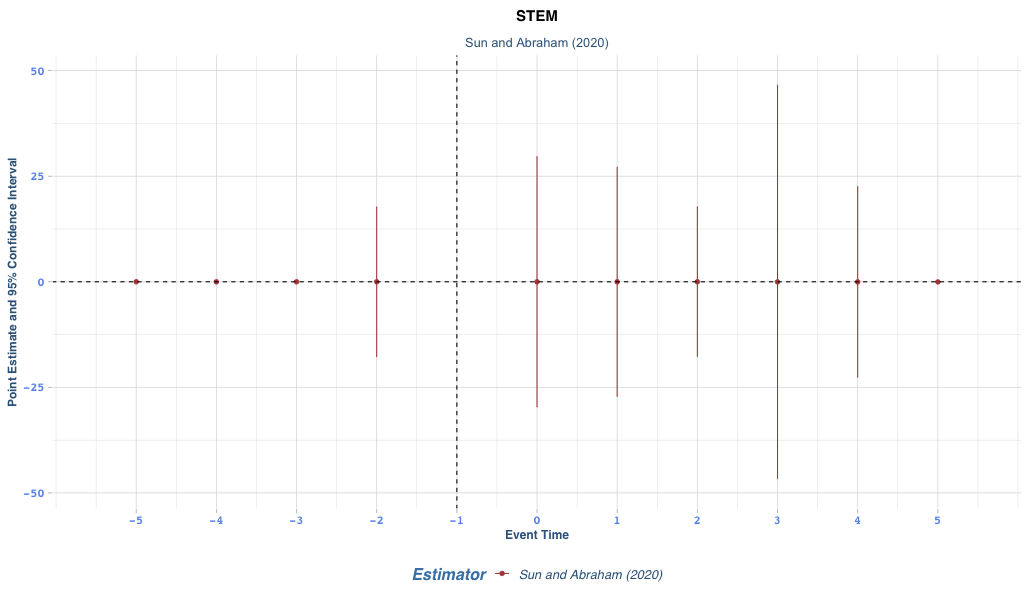
\includegraphics[width=\textwidth]{Graph/Results/stagered_ex_females_STEM.png}
        \caption{Proportion of Female Students Choosing STEM Majors in Schools Transitioning from Female to Coeducational}
    \label{fig:staggered_females_STEM}
\end{figure}

 
 

 
%%%%%%%%%%%%%%%%%%%%%%%%%%%%%%%%%%
 

  
 %%%%%%%%%%%%%%%%%%%%%%%%%%%%%%%%%%
\section{Conclusions} \label{section:05}

This study provides valuable insights into the impact of classroom gender composition on students' university major decisions. Our analysis reveals significant variations in female students' choices across academic disciplines, influenced by the presence of male peers in secondary school classrooms.

These findings underscore the complex interplay of gender dynamics in educational environments. Specifically, a higher proportion of male students correlates with increased interest among female students in traditionally male-dominated fields like engineering, architecture, and mathematics. Conversely, greater gender diversity in classrooms leads female students to exhibit a stronger preference for humanities and social sciences.

These results suggest that exposure to male peers may foster competitiveness and aspirations among female students, potentially narrowing gender gaps in STEM fields. However, they also highlight enduring gender-stereotypical preferences, with female students leaning towards communication-oriented disciplines in classrooms with more male representation.

Interestingly, minimal gender differences are observed in fields such as agriculture, veterinary sciences, and medicine, indicating limited influence of classroom gender compositions on major selection within these domains.

The findings underscore the importance of early educational experiences in shaping career trajectories and addressing gender disparities. By cultivating inclusive and gender-balanced learning environments, educational institutions can mitigate stereotypical pressures and promote equitable distribution of interests among students.

Moving forward, further research is warranted to elucidate the multifaceted mechanisms underlying these patterns, including peer influences, role modeling, and sociocultural norms. Longitudinal studies tracking students' evolving aspirations could provide deeper insights into the dynamics of gender composition and its long-term effects.

In conclusion, our analysis highlights the nuanced relationship between classroom gender composition and students' post-secondary schooling decisions. While specific majors exhibit varied responses to gender dynamics, overall, our findings suggest that gender-diverse environments may encourage female students to pursue higher education opportunities beyond secondary school.

%%%%%%%%%%%%%%%%%%%%%%%%%%%%%%%%%%
 
 
%%%%%%%%%%%%%%%%%%%%%%%%%%%%%%%%%%
  
 \newpage
\bibliographystyle{apacite}

\bibliography{Rereferences/bibliography}

\appendix 
\newpage

\subsection{Results by Fields of Study}
The varying preferences of female students across different fields of study  in post-secondary schooling decisions can be illuminated by three key factors: social dynamics, role models and mentors, and perceived stereotypes and bias.

In areas such as Economics, Business, Social Sciences/Humanities, Education Sciences, Health Sciences (except Medicine), Medicine, and Law, female students exhibit a higher preference  (See more details on preferred majors for female students in Subsection \ref{subsec:prefered_female}). This preference may be influenced by the presence of supportive social dynamics within these fields, where female students feel a sense of belonging and encouragement. Additionally, the availability of visible role models and mentors in these disciplines could inspire female students to pursue further studies.

Conversely, in fields such as Engineering, Architecture, Mathematics and Natural Sciences, female students exhibit a lower preference, potentially influenced by entrenched stereotypes suggesting these disciplines are more suited for males(For further details, refer to Subsection \ref{subsec:less_preferred_female}).. This bias, compounded by the competitiveness often observed in male students, tends to favor the choice of STEM-related careers, further dissuading female participation.



Interestingly, some areas such as Fine Arts and Agronomy/Veterinary-related fields demonstrate a similar level of preference between male and female students(For more insights, refer to Subsection \ref{subsec:similar_preference}). This parity suggests that in disciplines where social dynamics are more balanced, and stereotypes and biases are less pronounced, both genders may feel equally encouraged to pursue further studies.


\subsubsection{Fields of Study  Preferred by Female Students} \label{subsec:prefered_female}
In this section, we analyze the fields of study  where female students demonstrate a higher preference compared to male students.

1. \textbf{Economics, Business and  Related Majors}: The \citet{SUN2021175} estimation, depicted in the figure \ref{fig:staggered_economics_business} illustrates that the change in gender at school apparently does not significantly affect the decision to participate in careers related to administration and economics. However, it is crucial to note, as mentioned previously, that this observation only reflects the minimum diversity compositions of the new gender in the former single-gender schools. Therefore, the study depicted in Figure  \ref{fig:economics_business_related} becomes essential, as it considers several gender compositions and their relationship on career choices.
 


\begin{figure}[H]
    \centering
    \begin{subfigure}[b]{0.45\textwidth}
        \centering
        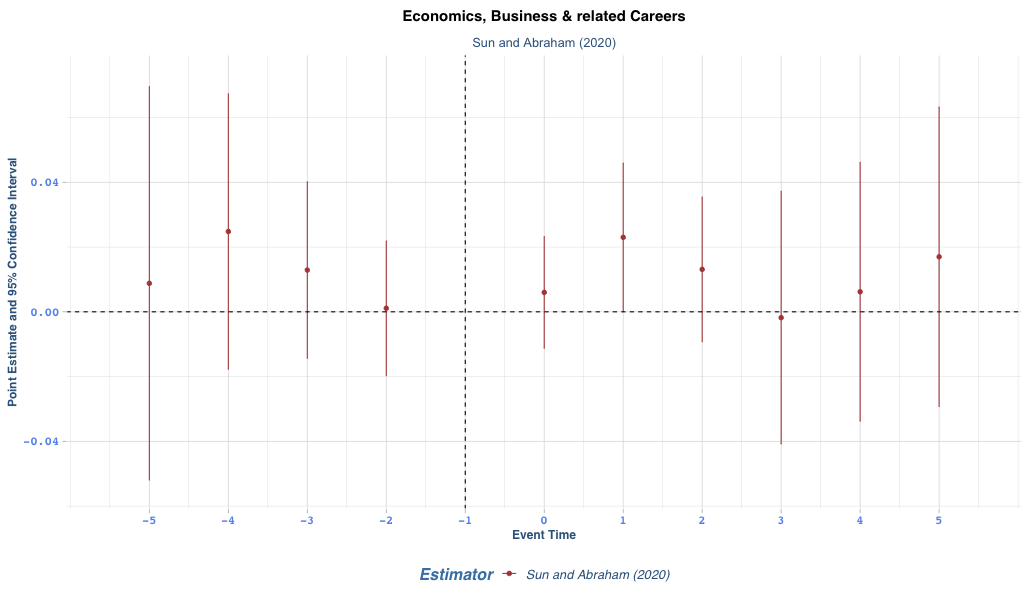
\includegraphics[width=\textwidth]{Graph/Results/stagered_ex_females_ECONOMICS_BUSINESS_RELATED.png}
        \caption{Ex female schools }
        \label{fig:staggered_females_economics_business}
    \end{subfigure}
    \hfill
    \begin{subfigure}[b]{0.45\textwidth}
        \centering
        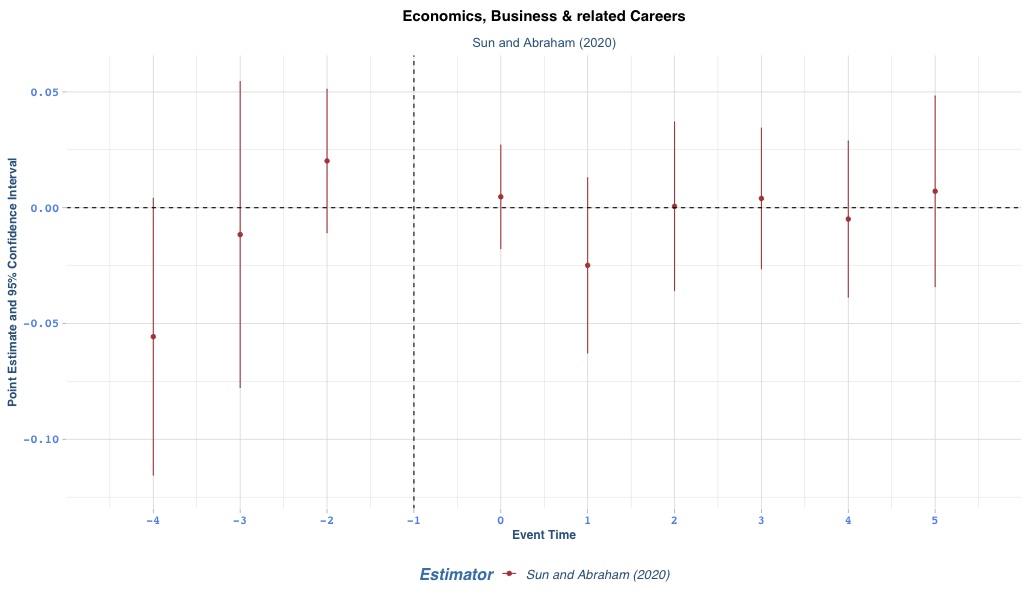
\includegraphics[width=\textwidth]{Graph/Results/stagered_ex_males_ECONOMICS_BUSINESS_RELATED.png}
        \caption{Ex male schools }
        \label{fig:staggered_males_economics_business}
    \end{subfigure}
\caption{ Changes in the Proportion of Students Choosing Economics and Business Related Majors in Schools Transitioning from Single-Sex to Coeducational}
    \label{fig:staggered_economics_business}
\end{figure}

The odds ratio for female students selecting majors in economics and business-related fields exhibits variation in response to changes in the male composition fraction within the classroom (See Figure \ref{fig:economics_business_related}).  As the proportion of male students increases, the odds ratio demonstrates fluctuation, reflecting the nuanced influence on female students' decisions regarding these majors. Higher proportions of male students in the classroom correlate with elevated odds ratios, suggesting a potential inclination among female students toward these majors in more gender-diverse environments. Notably, the analysis reveals that the odds ratio for the entire sample (12,120 students, depicted by the red line) peaks when the composition of male students in a classroom reaches approximately 29.22\%, with a substantial difference of 25 percentage points (0.64 - 0.39). This finding underscores the significant impact of classroom demographics on female students' preferences and underscores the importance of fostering gender diversity within educational settings.
 
\begin{figure}[H]
\centering
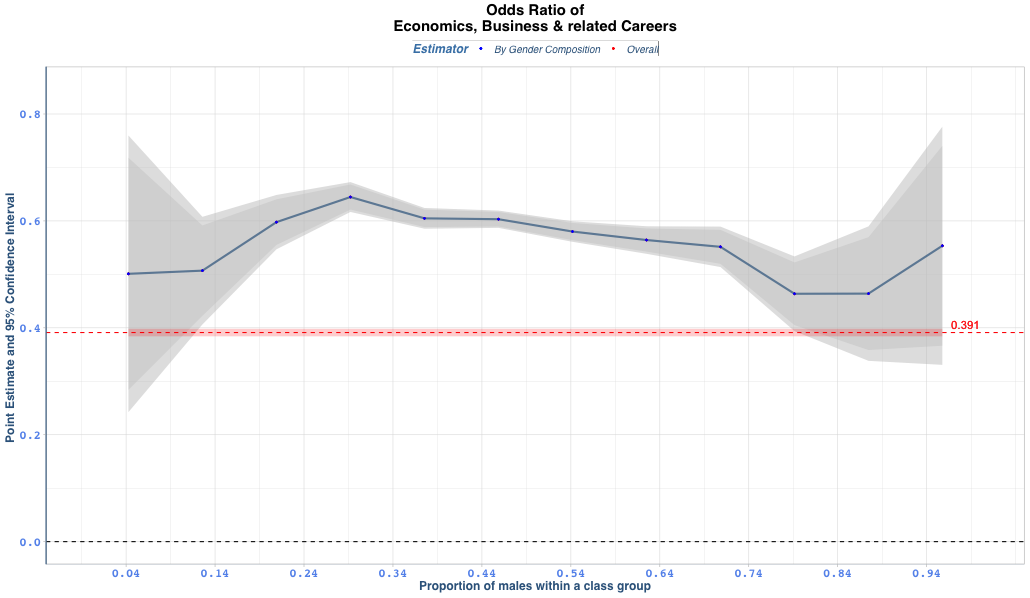
\includegraphics[width=0.8\textwidth]{Graph/Results/fe_panel_student_gender_composition_wome_in_ECONOMICS_BUSINESS_RELATED_bce.png}
\caption{Likelihood of a female student choosing economics/business-related majors}
\label{fig:economics_business_related}
\end{figure}

% Your analysis goes here


2. \textbf{Social Sciences/Humanities Majors}: The odds ratio for female students opting for majors in social sciences and humanities also varies with the male composition fraction in the classroom. Interestingly, unlike some other fields, higher proportions of male students are associated with higher odds ratios, indicating a potential preference among female students for these majors in more gender-diverse environments.

\begin{figure}[H]
    \centering
    \begin{subfigure}[b]{0.45\textwidth}
        \centering
        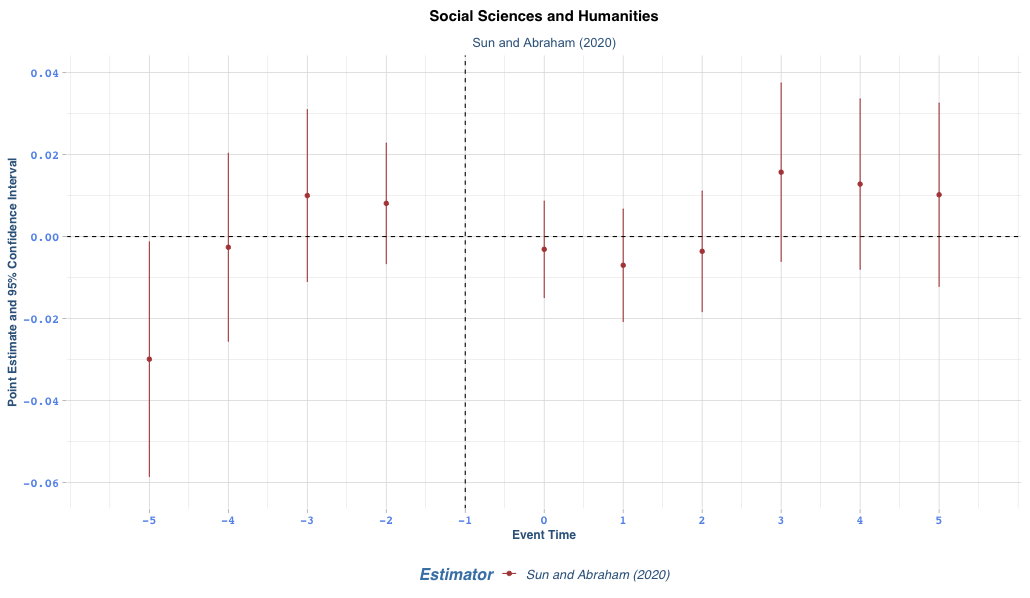
\includegraphics[width=\textwidth]{Graph/Results/stagered_ex_females_SOCIAL_SCIENCES_HUMANITIES.png}
        \caption{Ex female schools}
        \label{fig:staggered_females_social_sciences_humanities}
    \end{subfigure}
    \hfill
    \begin{subfigure}[b]{0.45\textwidth}
        \centering
        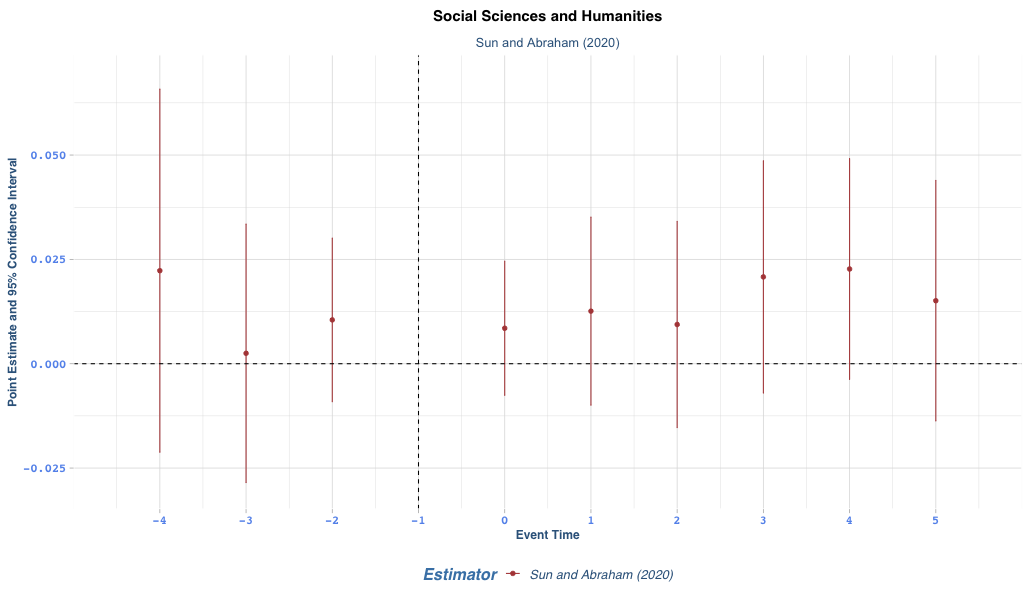
\includegraphics[width=\textwidth]{Graph/Results/stagered_ex_males_SOCIAL_SCIENCES_HUMANITIES.png}
        \caption{Ex male schools}
        \label{fig:staggered_males_social_sciences_humanities}
    \end{subfigure}
   \caption{ Changes in the Proportion of Students Choosing Social Sciences   in Schools Transitioning from Single-Sex to Coeducational}
    \label{fig:staggered_social_sciences_humanities}
\end{figure}


\begin{figure}[H]
\centering
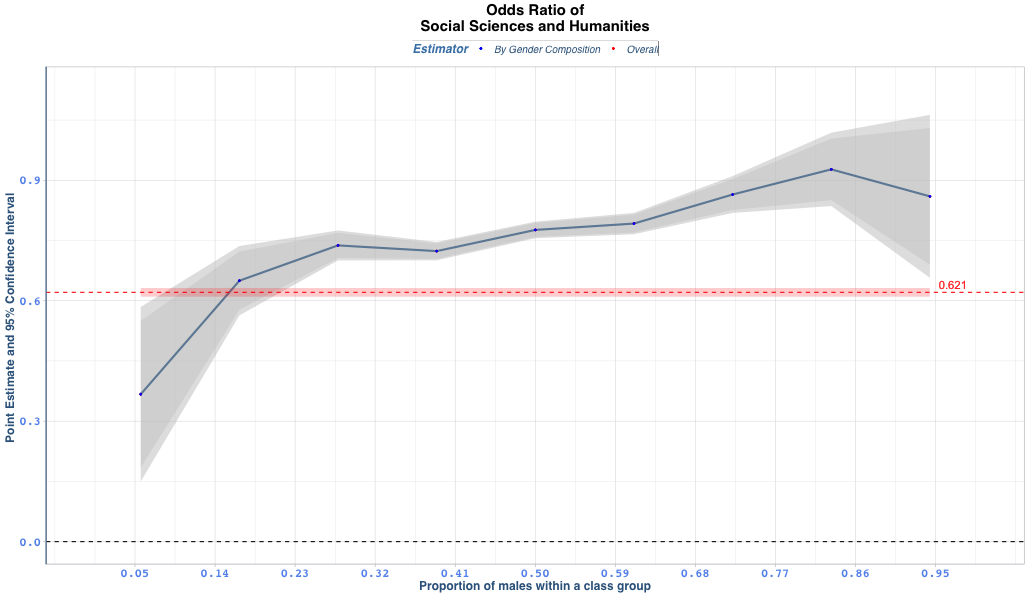
\includegraphics[width=0.8\textwidth]{Graph/Results/fe_panel_student_gender_composition_wome_in_SOCIAL_SCIENCES_HUMANITIES_bce.png}
\caption{Likelihood of a female student choosing social sciences/humanities majors}
\label{fig:social_sciences_humanities}
\end{figure}


3. \textbf{Education Sciences Majors}: The odds ratio for female students choosing majors in education sciences demonstrates variability based on the male composition fraction in the classroom. Interestingly, higher proportions of male students are associated with higher odds ratios, indicating a potential preference among female students for these majors in more gender-diverse environments.

\begin{figure}[H]
    \centering
    \begin{subfigure}[b]{0.45\textwidth}
        \centering
        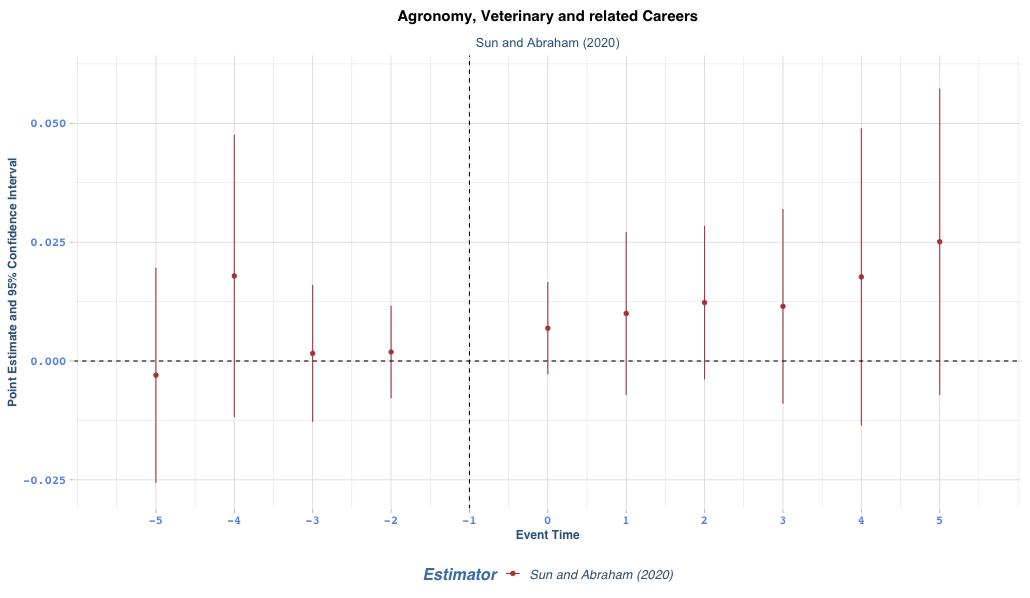
\includegraphics[width=\textwidth]{Graph/Results/stagered_ex_females_AGRONOMY_VETERINARY_RELATED.png}
        \caption{Ex female schools }
        \label{fig:staggered_females_education_sciences1}
    \end{subfigure}
    \hfill
    \begin{subfigure}[b]{0.45\textwidth}
        \centering
        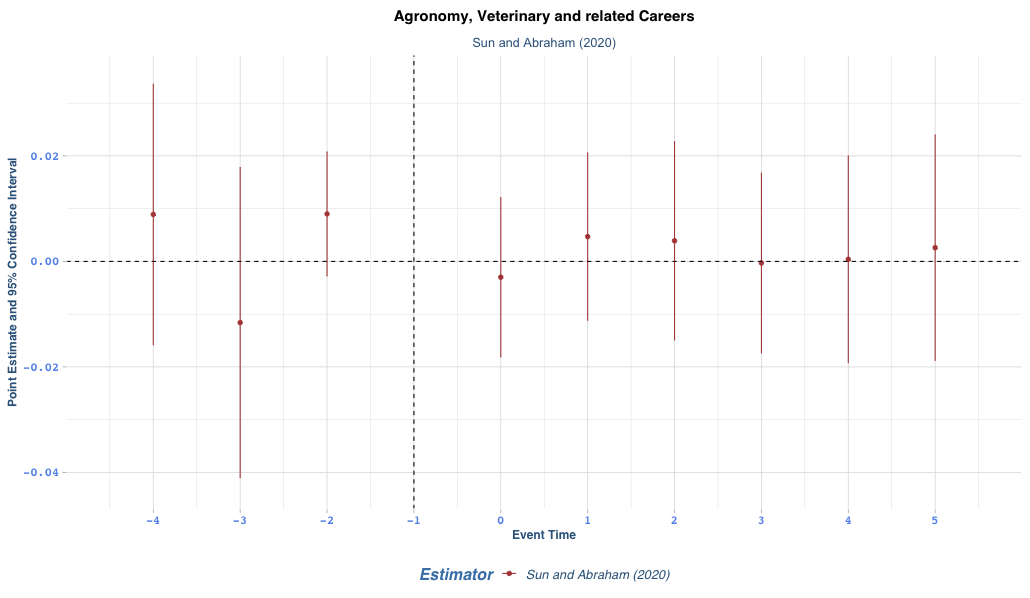
\includegraphics[width=\textwidth]{Graph/Results/stagered_ex_males_AGRONOMY_VETERINARY_RELATED.png}
        \caption{Ex male schools}
        \label{fig:staggered_males_education_sciences2}
    \end{subfigure}
       \caption{ Changes in the Proportion of Students Choosing Education Sciences Majors  in Schools Transitioning from Single-Sex to Coeducational}
    \label{fig:staggered_education_sciences1}
\end{figure}

\begin{figure}[H]
\centering
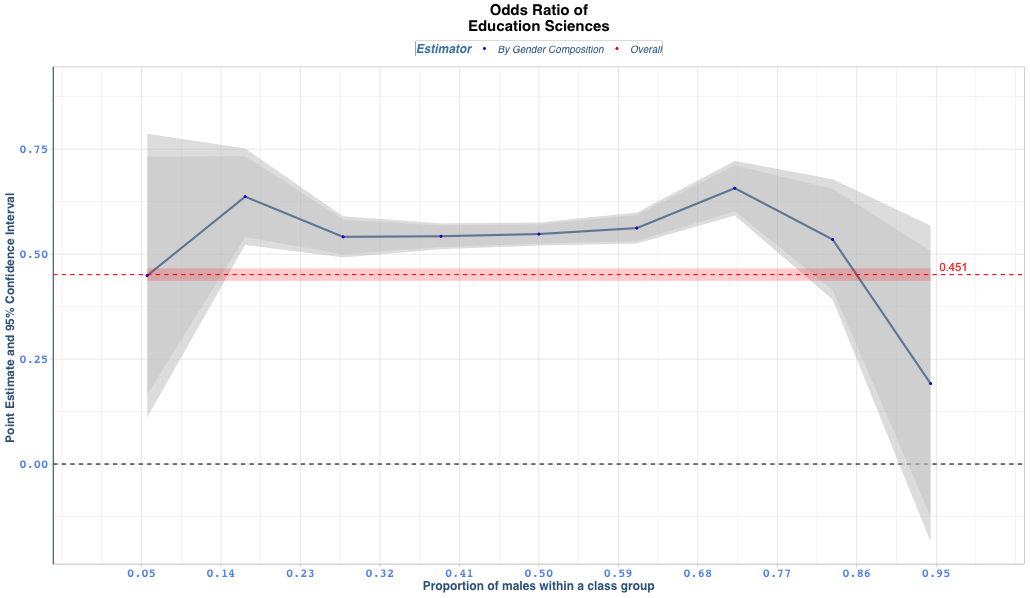
\includegraphics[width=0.8\textwidth]{Graph/Results/fe_panel_student_gender_composition_wome_in_EDUCATION_SCIENCES_bce.png}
\caption{Likelihood of a female student choosing education sciences majors}
\label{fig:education_sciences}
\end{figure}

4. \textbf{Health Sciences Majors (Except Medicine)}: The odds ratio for female students opting for majors in health sciences exhibits variability with changes in the male composition fraction in the classroom. Similar to some other fields, higher proportions of male students are associated with higher odds ratios, suggesting a potential preference among female students for these majors in more gender-diverse environments.

\begin{figure}[H]
    \centering
    \begin{subfigure}[b]{0.45\textwidth}
        \centering
        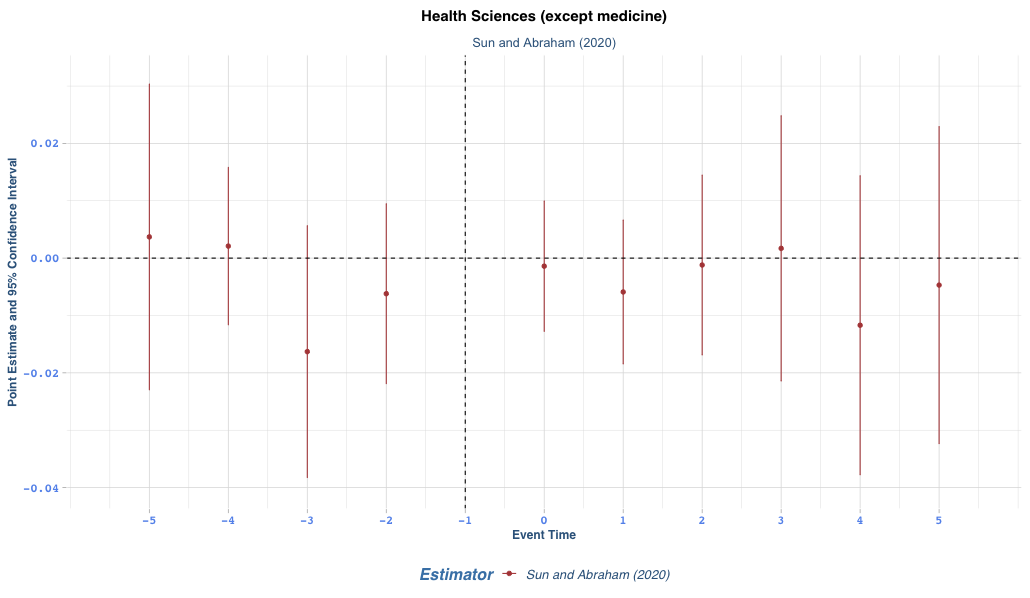
\includegraphics[width=\textwidth]{Graph/Results/stagered_ex_females_HEALTH_SCIENCES.png}
        \caption{Ex female schools }
        \label{fig:staggered_females_health_sciences}
    \end{subfigure}
    \hfill
    \begin{subfigure}[b]{0.45\textwidth}
        \centering
        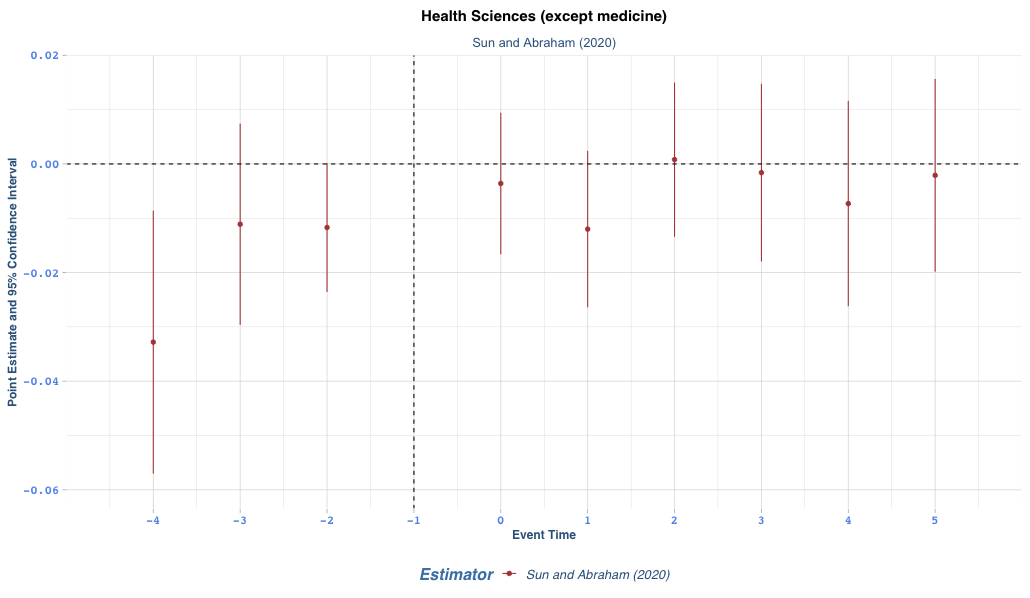
\includegraphics[width=\textwidth]{Graph/Results/stagered_ex_males_HEALTH_SCIENCES.png}
        \caption{Ex male schools}
        \label{fig:staggered_males_health_sciences}
    \end{subfigure}
       \caption{ Changes in the Proportion of Students Choosing Health Science Majors (Except Medicine) in Schools Transitioning from Single-Sex to Coeducational}
    \label{fig:staggered_health_sciences}
\end{figure}

\begin{figure}[H]
\centering
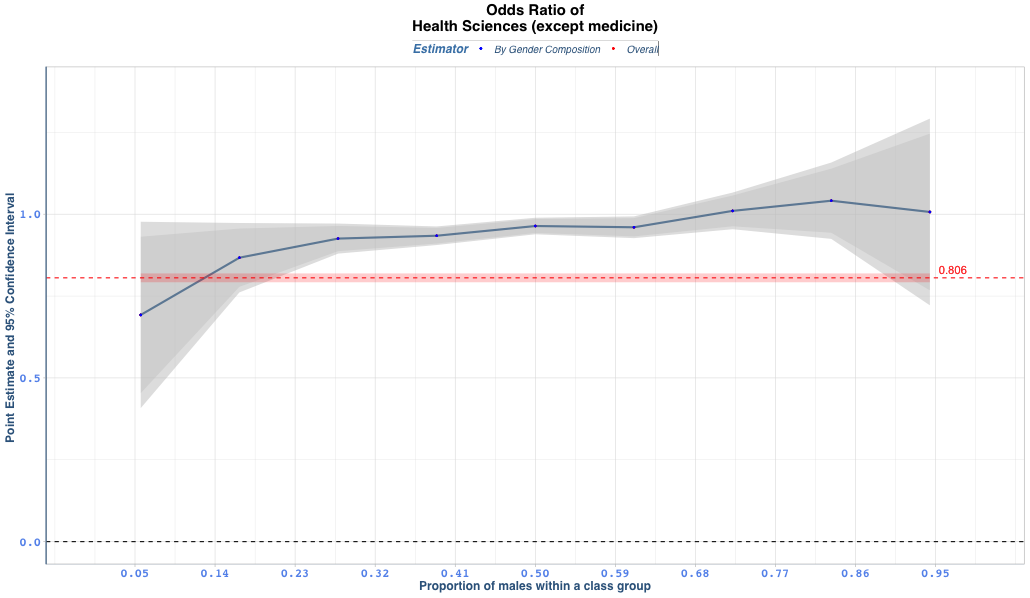
\includegraphics[width=0.8\textwidth]{Graph/Results/fe_panel_student_gender_composition_wome_in_HEALTH_SCIENCES_bce.png}
\caption{Likelihood of a female student choosing health sciences majors}
\label{fig:health_sciences}
\end{figure}




5. \textbf{Medicine Major}: The odds ratio for female students selecting majors in medicine fluctuates with changes in the male composition fraction in the classroom. Higher proportions of male students are associated with lower odds ratios, suggesting potential barriers or deterrents for female students in pursuing medicine majors in more male-dominated environments.

\begin{figure}[H]
    \centering
    \begin{subfigure}[b]{0.45\textwidth}
        \centering
        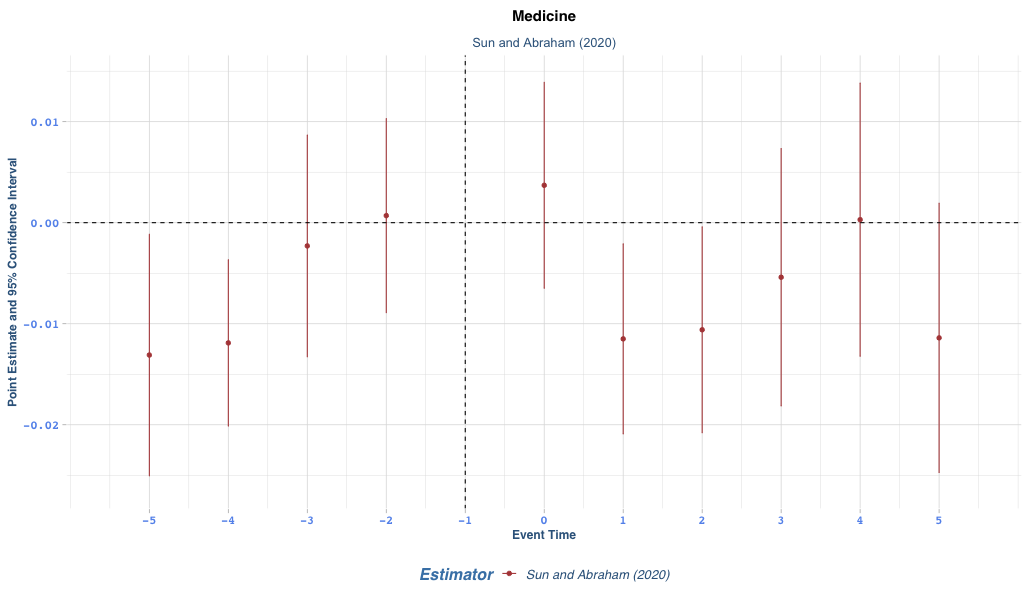
\includegraphics[width=\textwidth]{Graph/Results/stagered_ex_females_MEDICINE.png}
        \caption{Ex female schools }
        \label{fig:staggered_females_medicine}
    \end{subfigure}
    \hfill
    \begin{subfigure}[b]{0.45\textwidth}
        \centering
        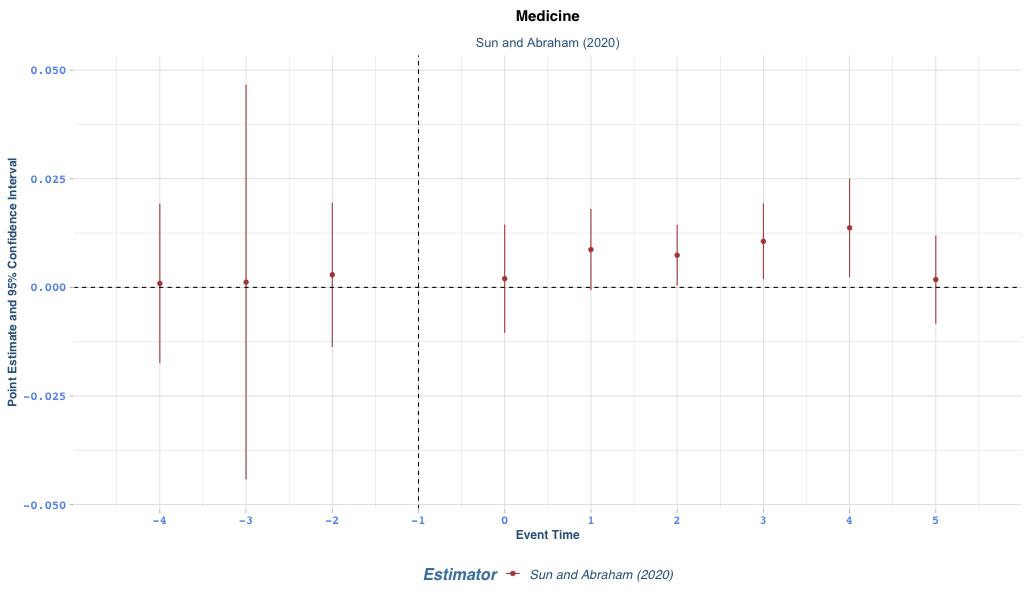
\includegraphics[width=\textwidth]{Graph/Results/stagered_ex_males_MEDICINE.png}
        \caption{Ex male schools}
        \label{fig:staggered_males_medicine}
    \end{subfigure}
       \caption{ Changes in the Proportion of Students Choosing A Major in Medicine from Schools Transitioning from Single-Sex to Coeducational}
    \label{fig:staggered_medicine}
\end{figure}

\begin{figure}[H]
\centering
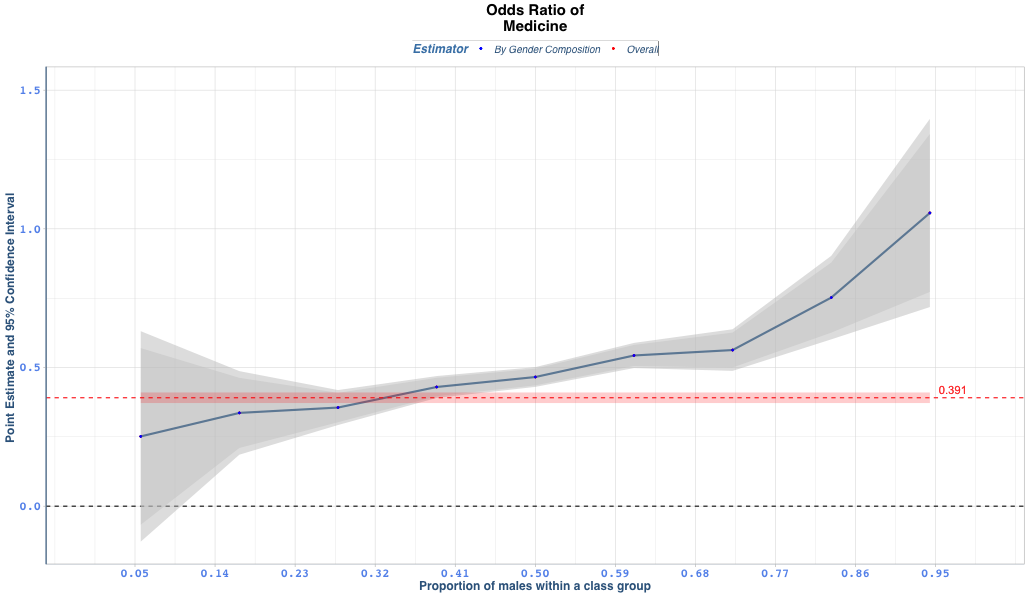
\includegraphics[width=0.8\textwidth]{Graph/Results/fe_panel_student_gender_composition_wome_in_MEDICINE_bce.png}
\caption{Likelihood of a female student choosing medicine majors}
\label{fig:medicine}
\end{figure}

6. \textbf{Law Majors}: The odds ratio for female students opting for majors in law demonstrates variability with changes in the male composition fraction in the classroom. Higher proportions of male students are associated with higher odds ratios, suggesting a potential preference among female students for these majors in more gender-diverse environments.

\begin{figure}[H]
    \centering
    \begin{subfigure}[b]{0.45\textwidth}
        \centering
        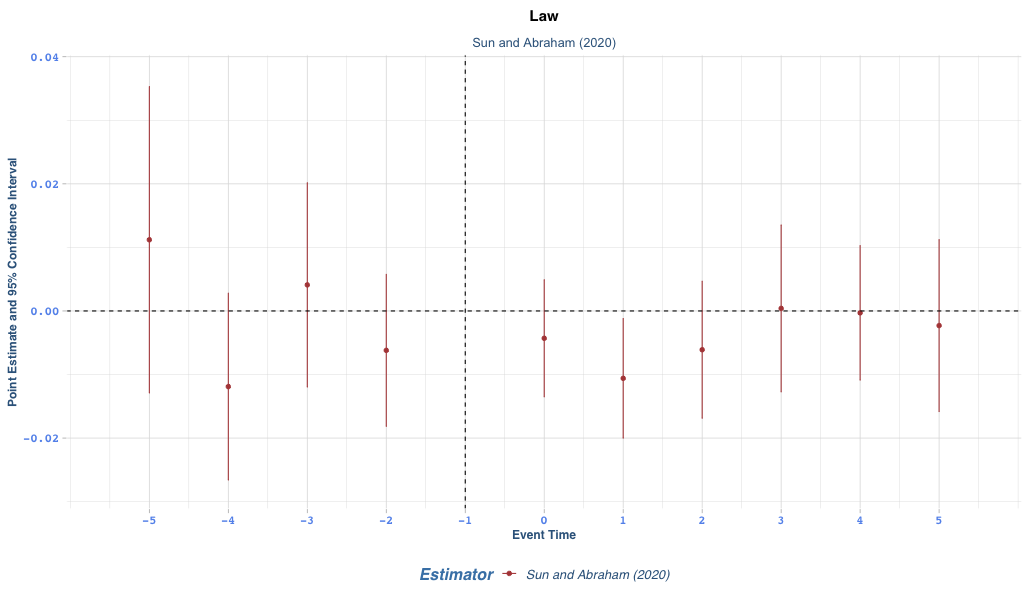
\includegraphics[width=\textwidth]{Graph/Results/stagered_ex_females_LAW.png}
        \caption{Ex female schools }
        \label{fig:staggered_females_education_sciences}
    \end{subfigure}
    \hfill
    \begin{subfigure}[b]{0.45\textwidth}
        \centering
        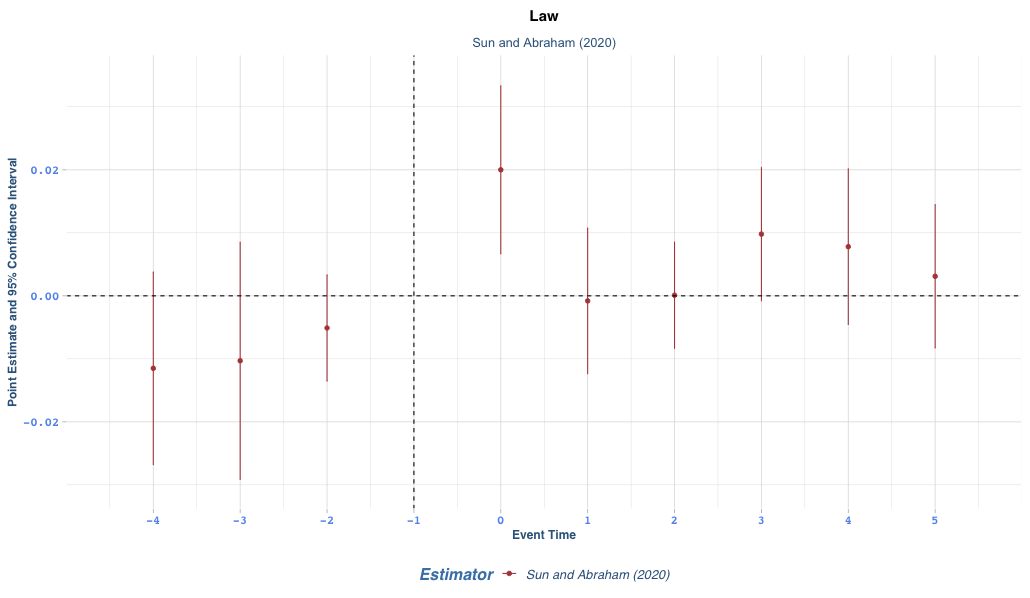
\includegraphics[width=\textwidth]{Graph/Results/stagered_ex_males_LAW.png}
        \caption{Ex male schools}
        \label{fig:staggered_males_education_sciences}
    \end{subfigure}
       \caption{ Changes in the Proportion of Students Choosing  a Major in LAW in Schools Transitioning from Single-Sex to Coeducational}
    \label{fig:staggered_education_sciences}
\end{figure}

\begin{figure}[htbp]
\centering
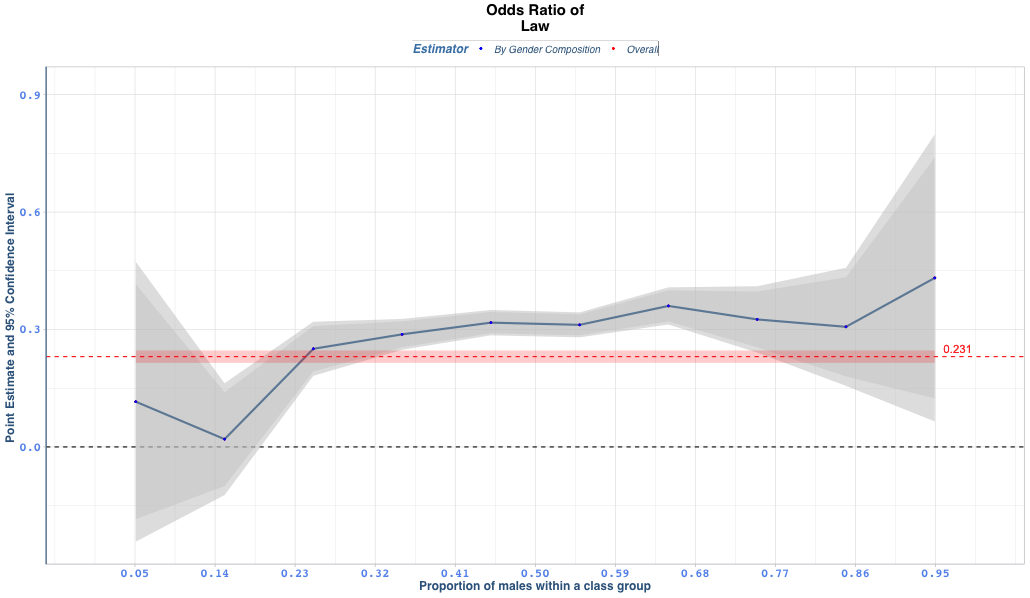
\includegraphics[width=0.8\textwidth]{Graph/Results/fe_panel_student_gender_composition_wome_in_LAW_bce.png}
\caption{Likelihood of a female student choosing law majors}
\label{fig:law}
\end{figure}

\subsubsection{Fields of Study  Less Preferred by Female Students}\label{subsec:less_preferred_female}

This section examines the fields of study  where female students display a lower preference compared to male students.



 


1. \textbf{Engineering/Architecture Related Majors}: The odds ratio for female students opting for majors in engineering and architecture also exhibits variability based on the male composition fraction in the classroom. Interestingly, as the proportion of male students increases, the odds ratio tends to decrease, suggesting a potential deterrent effect on female students' interest in these fields. This trend highlights the importance of considering classroom demographics in understanding gender disparities in engineering and architecture-related majors.

 
\begin{figure}[H]
    \centering
    \begin{subfigure}[b]{0.45\textwidth}
        \centering
        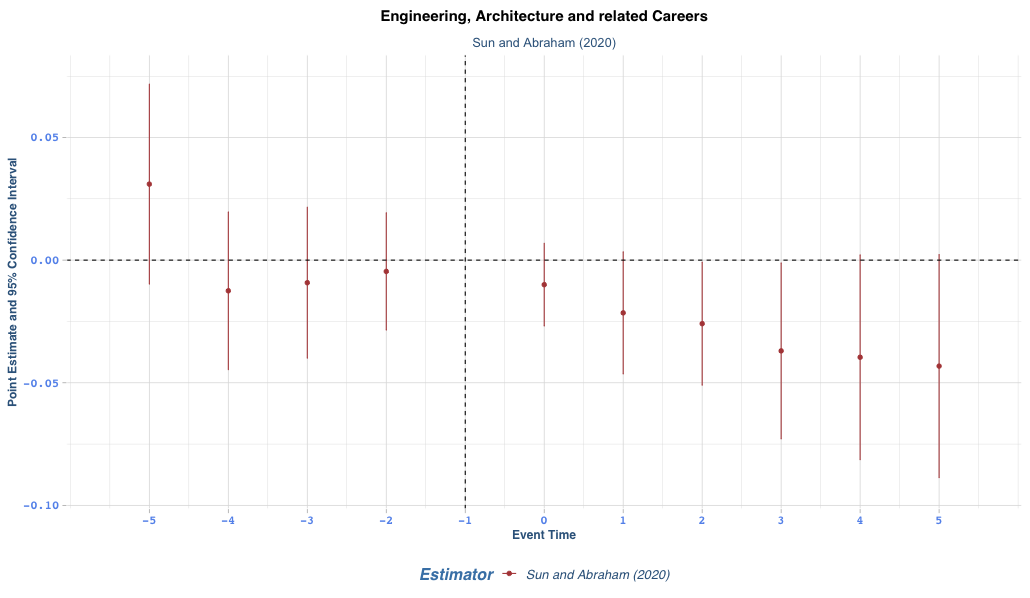
\includegraphics[width=\textwidth]{Graph/Results/stagered_ex_females_ENG_ARCH_RELATED.png}
        \caption{Ex female schools }
        \label{fig:staggered_females_eng}
    \end{subfigure}
    \hfill
    \begin{subfigure}[b]{0.45\textwidth}
        \centering
        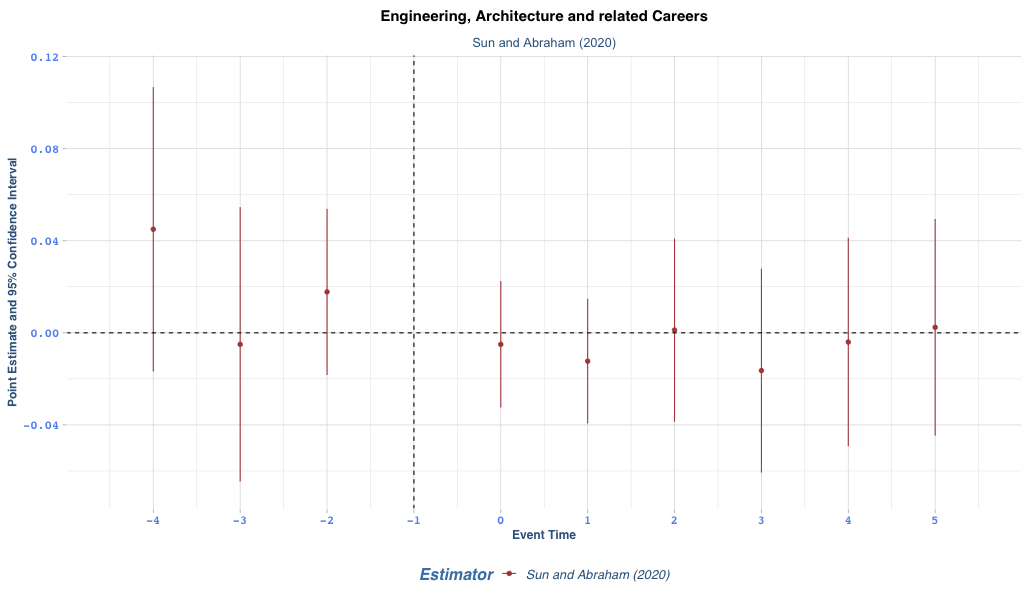
\includegraphics[width=\textwidth]{Graph/Results/stagered_ex_males_ENG_ARCH_RELATED.png}
        \caption{Ex male schools }
        \label{fig:staggered_males_eng}
    \end{subfigure}
\caption{ Changes in the Proportion of Students Choosing Engineering, Architecture and  Related Majors in Schools Transitioning from Single-Sex to Coeducational}
    \label{fig:staggered_eng_arch_related}
\end{figure}

\begin{figure}[H]
\centering
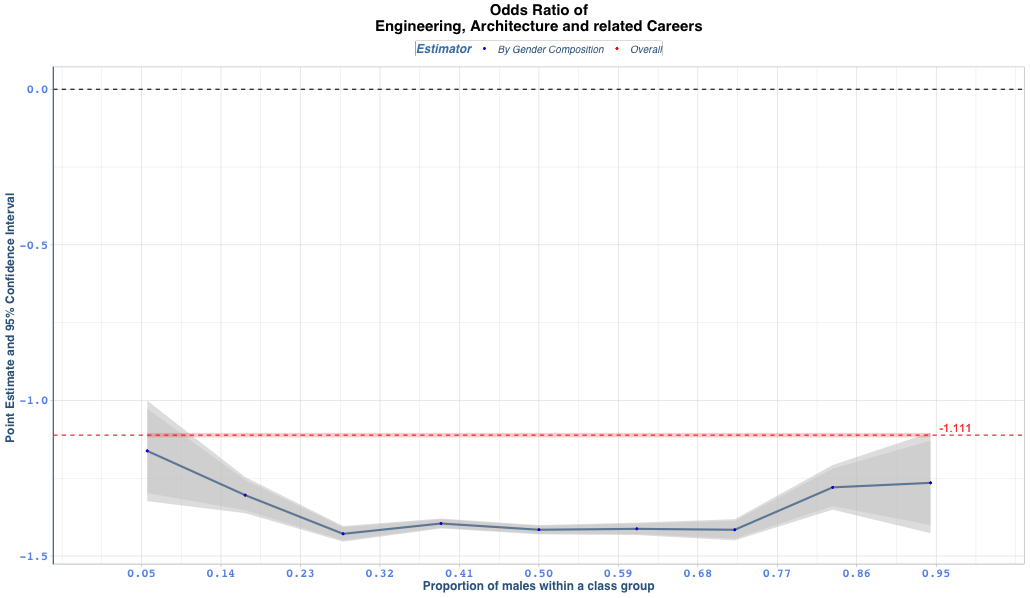
\includegraphics[width=0.8\textwidth]{Graph/Results/fe_panel_student_gender_composition_wome_in_ENG_ARCH_RELATED_bce.png}
\caption{Likelihood of a female student choosing engineering/architecture-related majors}
\label{fig:eng_arch_related}
\end{figure}

% Your analysis goes here

2. \textbf{Mathematics and Natural Sciences Majors}: Similar to other fields, the odds ratio for female students selecting majors in mathematics and natural sciences fluctuates with changes in the male composition fraction. Higher proportions of male students in the classroom are associated with lower odds ratios, suggesting potential barriers or deterrents for female students in pursuing these majors in more male-dominated environments.

\begin{figure}[H]
    \centering
    \begin{subfigure}[b]{0.45\textwidth}
        \centering
        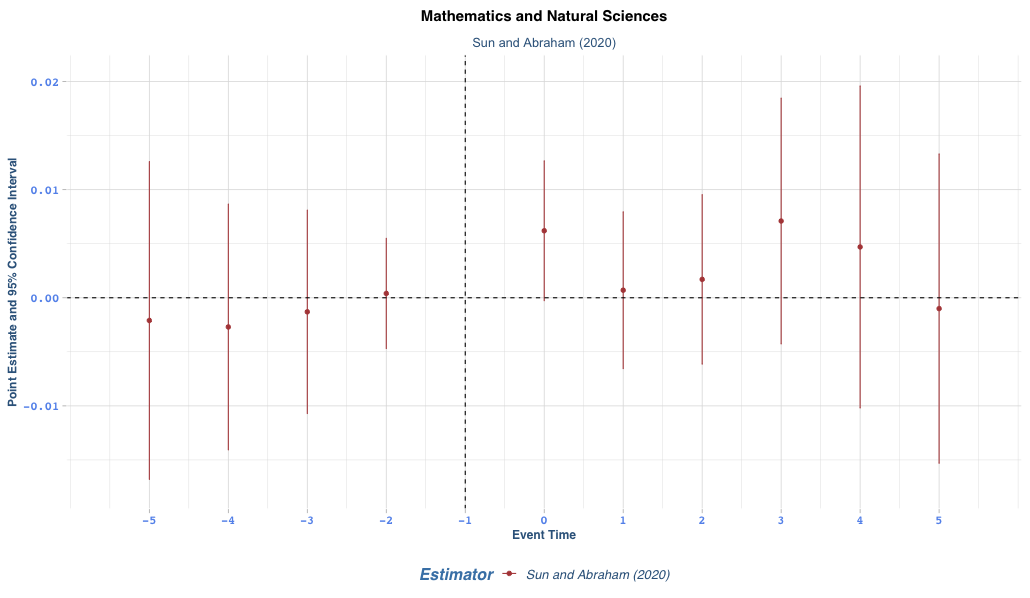
\includegraphics[width=\textwidth]{Graph/Results/stagered_ex_females_MATHEMATICS_NATURAL_SCIENCES.png}
        \caption{Ex female schools }
        \label{fig:staggered_females_math_natural_sciences}
    \end{subfigure}
    \hfill
    \begin{subfigure}[b]{0.45\textwidth}
        \centering
        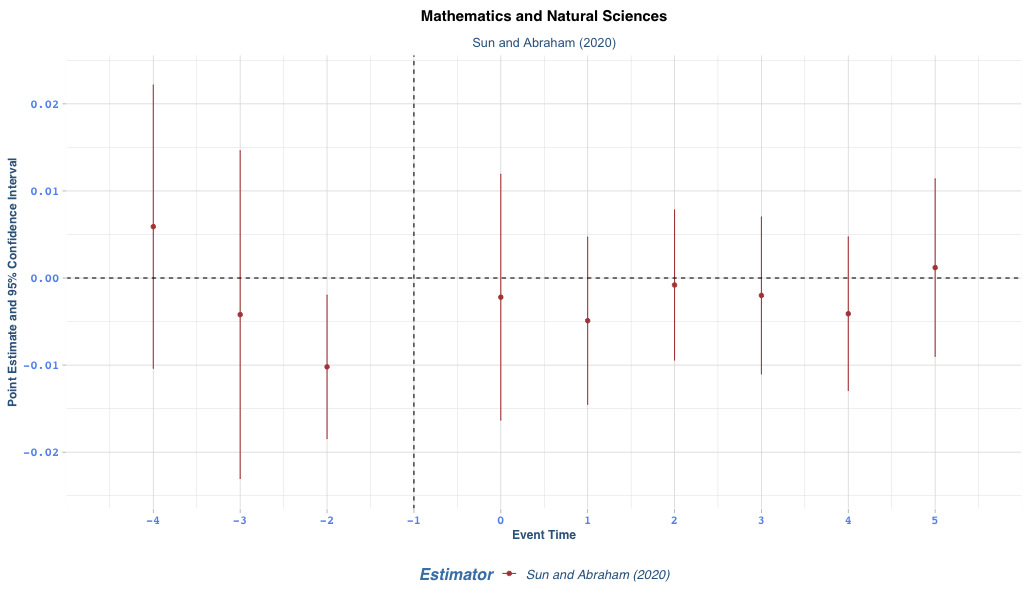
\includegraphics[width=\textwidth]{Graph/Results/stagered_ex_males_MATHEMATICS_NATURAL_SCIENCES.png}
        \caption{Ex male schools }
        \label{fig:staggered_males_math_natural_sciences}
    \end{subfigure}
\caption{ Changes in the Proportion of Students Choosing Mathematics, Natural Sciences and Related Majors   in Schools Transitioning from Single-Sex to Coeducational}
    \label{fig:staggered_math_natural_sciences}
\end{figure}

\begin{figure}[H]
\centering
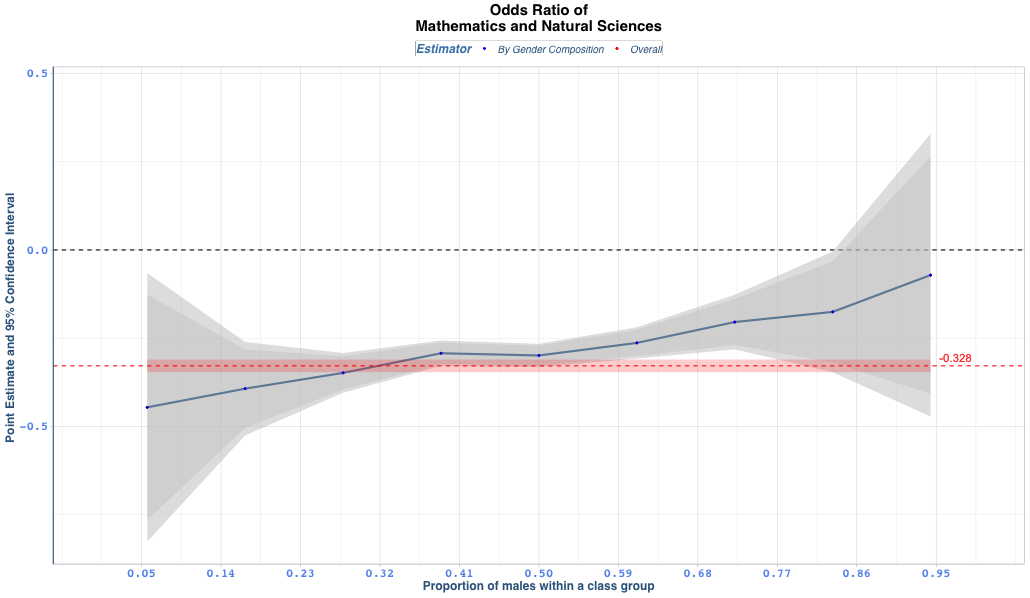
\includegraphics[width=0.8\textwidth]{Graph/Results/fe_panel_student_gender_composition_wome_in_MATHEMATICS_NATURAL_SCIENCES_bce.png}
\caption{Likelihood of a female student choosing mathematics/natural sciences majors}
\label{fig:math_natural_sciences}
\end{figure}



\subsubsection{Fields of Study  with Similar Preferences Between Female and Male Students}\label{subsec:similar_preference}

Here, we explore the fields of study  where both female and male students exhibit similar preferences.
 

 
1. \textbf{Fine Arts Majors}: The odds ratio for female students choosing majors in fine arts demonstrates a less consistent pattern compared to other fields. While there is some fluctuation in the odds ratio with changes in the male composition fraction, the overall trend is less pronounced. Female students seem to exhibit varying preferences for fine arts majors regardless of the gender composition in the classroom.

\begin{figure}[H]
    \centering
    \begin{subfigure}[b]{0.45\textwidth}
        \centering
        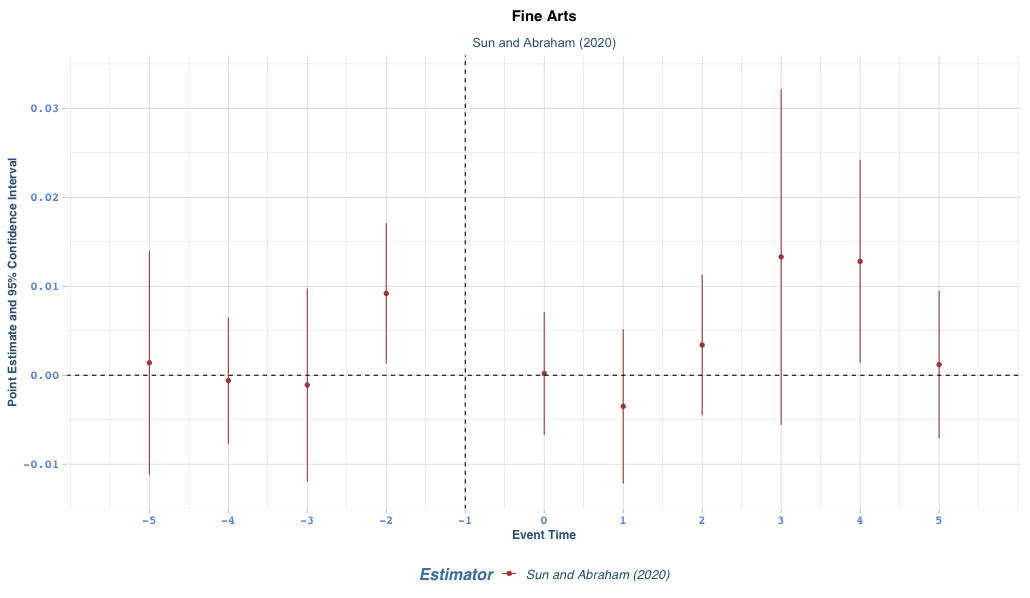
\includegraphics[width=\textwidth]{Graph/Results/stagered_ex_females_FINE_ARTS.png}
        \caption{Ex female schools }
        \label{fig:staggered_females_fine_arts}
    \end{subfigure}
    \hfill
    \begin{subfigure}[b]{0.45\textwidth}
        \centering
        \includegraphics[width=\textwidth]{Graph/Results/stagered_ex_Males_FINE_ARTS.png}
        \caption{Ex male schools }
        \label{fig:staggered_males_fine_arts}
    \end{subfigure}
\caption{ Changes in the Proportion of Students Choosing Fine Arts and Related Majors in Schools Transitioning from Single-Sex to Coeducational}
    \label{fig:staggered_fine_arts}
\end{figure}

\begin{figure}[H]
\centering
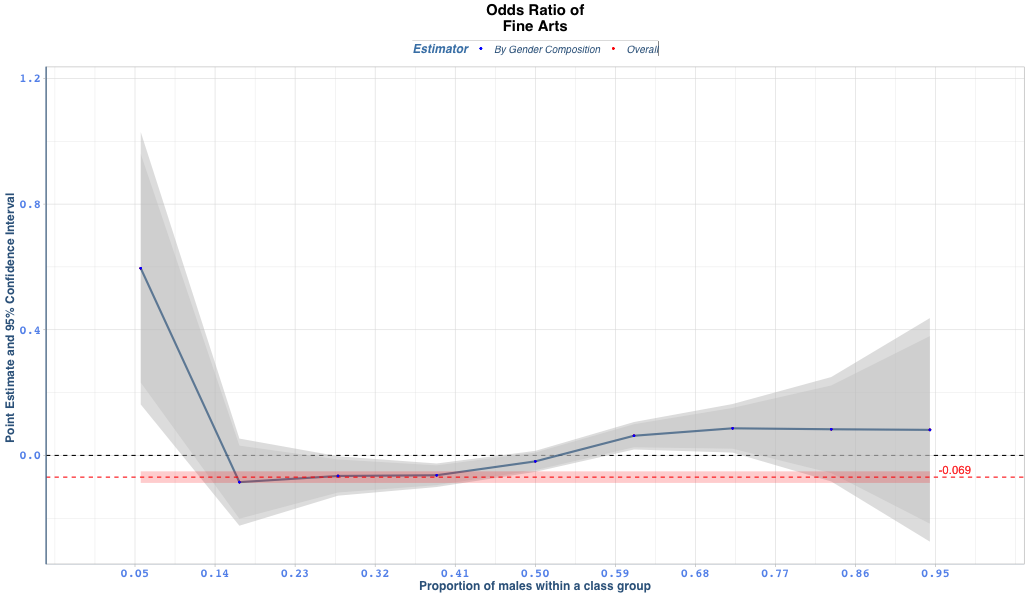
\includegraphics[width=0.8\textwidth]{Graph/Results/fe_panel_student_gender_composition_wome_in_FINE_ARTS_bce.png}
\caption{Likelihood of a female student choosing fine arts majors}
\label{fig:fine_arts}
\end{figure}

2. \textbf{Agronomy/Veterinary Related Majors}: The odds ratio for female students selecting majors in agronomy and veterinary-related fields shows fluctuations with changes in the male composition fraction in the classroom. Higher proportions of male students are associated with lower odds ratios, suggesting potential barriers or deterrents for female students in pursuing these majors in more male-dominated environments.

 
\begin{figure}[H]
    \centering
    \begin{subfigure}[b]{0.45\textwidth}
        \centering
        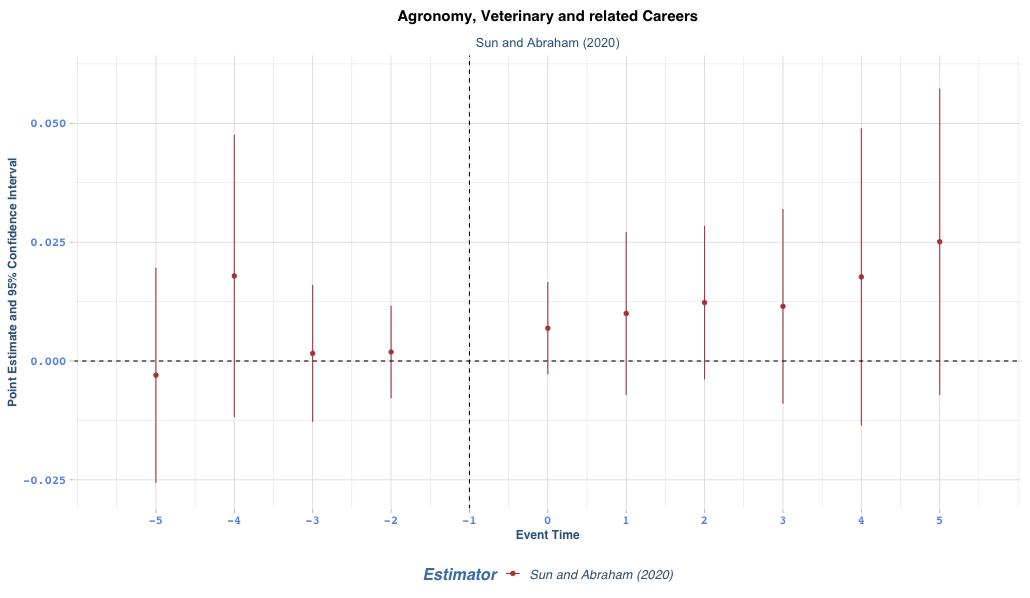
\includegraphics[width=\textwidth]{Graph/Results/stagered_ex_females_AGRONOMY_VETERINARY_RELATED.png}
        \caption{Ex female schools }
        \label{fig:staggered_females_agronomy_veterinary}
    \end{subfigure}
    \hfill
    \begin{subfigure}[b]{0.45\textwidth}
        \centering
        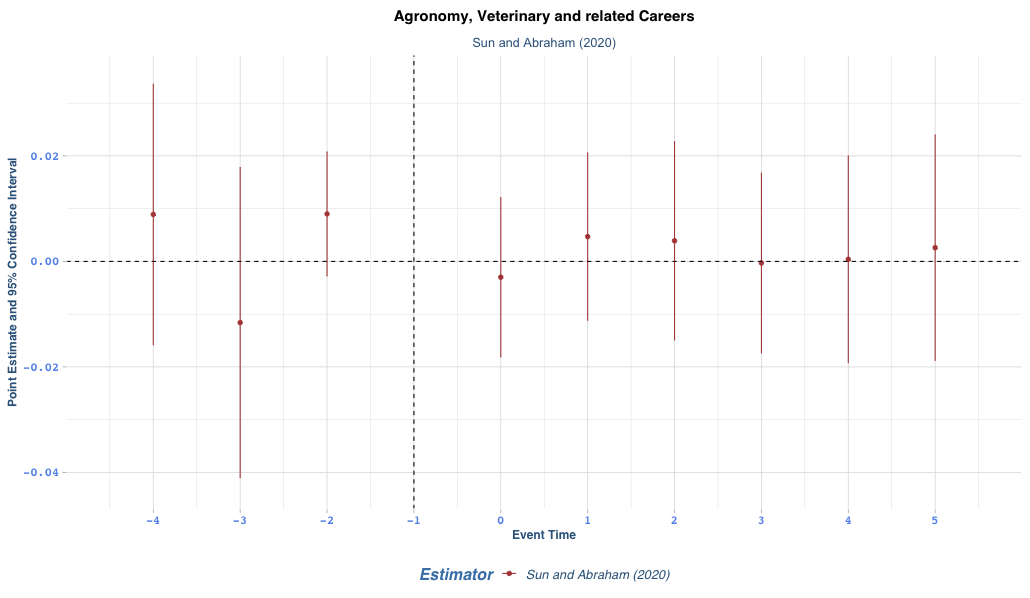
\includegraphics[width=\textwidth]{Graph/Results/stagered_ex_males_AGRONOMY_VETERINARY_RELATED.png}
        \caption{Ex male schools}
        \label{fig:staggered_males_agronomy_veterinary}
    \end{subfigure}
       \caption{ Changes in the Proportion of Students Choosing Agronomy, Veterinary, and Related Majors in Schools Transitioning from Single-Sex to Coeducational}
    \label{fig:staggered_agronomy_veterinary}
\end{figure}


 
\begin{figure}[H]
\centering
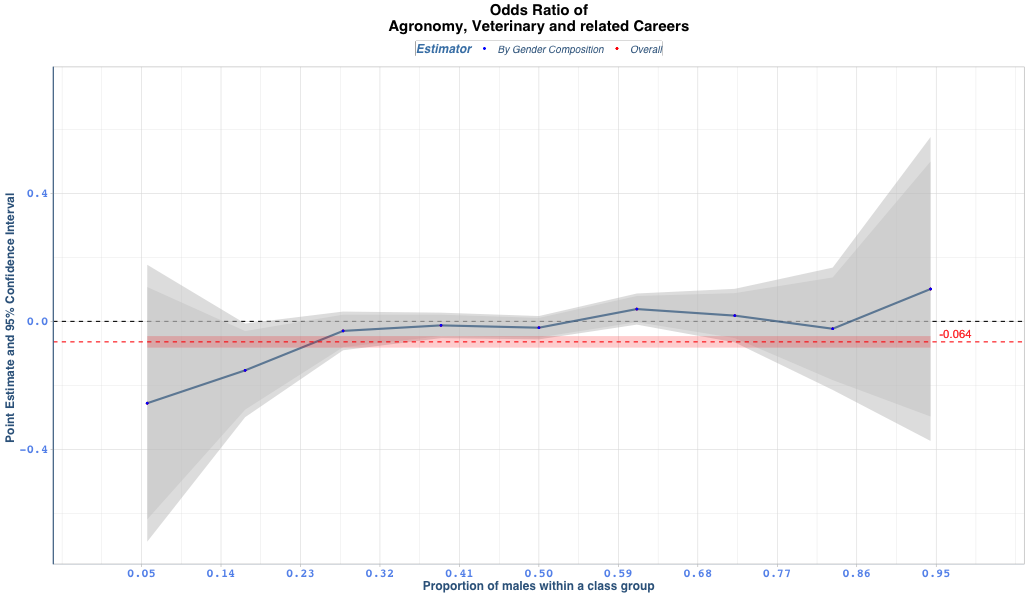
\includegraphics[width=0.8\textwidth]{Graph/Results/fe_panel_student_gender_composition_wome_in_AGRONOMY_VETERINARY_RELATED_bce.png}
\caption{Likelihood of a female student choosing agronomy/veterinary-related majors}
\label{fig:agronomy_veterinary_related}
\end{figure}

% \subsection{-----}
\subsection{Description of University Major Choices by Knowledge Areas} \label{app:path}

This section provides an overview of university major choices categorized into distinct knowledge areas. The aggregated classification is structured as follows:
    \begin{itemize}
        \item 1. Economics, Business \& related Careers ( e.g., Economics, Business Administration, Finance, Accounting, Marketing, Management, Entrepreneurship, International Business, Human Resources)
        \item 2. Engineering, Architecture \ and related Careers (e.g., Civil Engineering, Mechanical Engineering, Electrical Engineering, Architecture, Computer Science, Information Technology, Software Engineering, Industrial Design, Environmental Engineering, Biomedical Engineering)
        \item 3. Fine Arts (Visual Arts, Performing Arts (e.g., Theater, Dance, Music), Graphic Design, Interior Design, Animation)
        \item 4. Mathematics and Natural Sciences (e.g., Mathematics, Physics, Chemistry, Biology, Environmental Science, Geology, Astronomy, Statistics)
        \item 5. Social Sciences and Humanities (e.g.,  Sociology, Anthropology, History, Political Science, Geography, Literature, Philosophy, Religious Studies, Linguistics, Communication Studies)
        \item 6. Agronomy, Veterinary \ and related Careers (e.g., Agronomy, Animal Science, Veterinary Medicine, Zoology, Horticulture, Fisheries and Aquaculture)
        \item 7. Education Sciences (e.g.,  Early Childhood Education, Special Education, Educational Psychology, Education in Mathematics, Education in Sciences ) 
        \item 8. Health Sciences (e.g.,  Nursing, Dentistry, Pharmacy, Physical Therapy, Occupational Therapy, Public Health, Nutrition, Biomedical Sciences, Health Administration,)
        \item 9. No Studies (The student does not continue with professional studies)
    \end{itemize}
\begin{table}[!htbp]
  \centering
  \caption{Correlation between Gender Composition in a Class and Likelihood of Choosing a Career}
  \label{tab:tab1}
  \begin{tabular}{lcccccccccc}
    \toprule
    & \multicolumn{9}{c}{\textit{Dependent variable: Likelihood of Choosing Career}} \\
    \cmidrule(lr){2-10} 
    & (1) & (2) & (3) & (4) & (5) & (6) & (7) & (8) & (9) \\
    \midrule
    Proportion of Males & -0.931*** & 0.982*** & -0.200*** & -0.436*** & -0.996*** & -0.011 & -0.707*** & -1.119*** & 0.445*** \\
    & (0.010) & (0.009) & (0.026) & (0.026) & (0.012) & (0.026) & (0.021) & (0.015) & (0.006) \\
    \addlinespace
    Constant & -1.828*** & -2.535*** & -4.285*** & -4.176*** & -2.407*** & -4.335*** & -3.658*** & -2.732*** & 0.385*** \\
    & (0.005) & (0.005) & (0.013) & (0.012) & (0.006) & (0.012) & (0.010) & (0.007) & (0.003) \\
    \midrule
    Observations & \multicolumn{1}{c}{4,486,601} & \multicolumn{1}{c}{4,486,601} & \multicolumn{1}{c}{4,486,601} & \multicolumn{1}{c}{4,486,601} & \multicolumn{1}{c}{4,486,601} & \multicolumn{1}{c}{4,486,601} & \multicolumn{1}{c}{4,486,601} & \multicolumn{1}{c}{4,486,601} & \multicolumn{1}{c}{4,486,601} \\
    Log Likelihood & \multicolumn{1}{c}{-1,412,835.0} & \multicolumn{1}{c}{-1,562,897.0} & \multicolumn{1}{c}{-299,879.8} & \multicolumn{1}{c}{-300,436.7} & \multicolumn{1}{c}{-947,917.1} & \multicolumn{1}{c}{-308,616.4} & \multicolumn{1}{c}{-411,800.1} & \multicolumn{1}{c}{-723,508.2} & \multicolumn{1}{c}{-2,921,328.0} \\
    AIC & \multicolumn{1}{c}{2,825,674.0} & \multicolumn{1}{c}{3,125,798.0} & \multicolumn{1}{c}{599,763.7} & \multicolumn{1}{c}{600,877.4} & \multicolumn{1}{c}{1,895,838.0} & \multicolumn{1}{c}{617,236.9} & \multicolumn{1}{c}{823,604.2} & \multicolumn{1}{c}{1,447,020.0} & \multicolumn{1}{c}{5,842,660.0} \\
    \bottomrule
  \end{tabular}
\begin{threeparttable}
  \begin{tablenotes}
  \small
    \item Note: $^{*}$p$<$0.1; $^{**}$p$<$0.05; $***$p$<$0.01 
  \end{tablenotes}
  \end{threeparttable}
\end{table}

\newpage
 \subsection{Optimal bandwidth estimation based on Binary cross-entropy }
 \label{bce}

In order to analyze the probability that a secondary school student chooses an field of study  $P$ to pursue post-secondary studies. We analyze the probability according to different gender compositions in the classrooms. Therefore we assume that exists a fixed value that allow to subset by $\exists X_{\text{optimal}}$  The formal representation using mathematical notation for the partitioning of the range into fixed intervals:
Let $X_i$ be a subset that belongs to the gender composition with values between [0,1], we can say that, $X_1$ is a subset that goes from $\min(X)$ to $\min(X)$+$X_i$, consequently $X_2$ is a subset which goes from $X_1$ to $X_1$+$X_i$, and sequentially until $X_n$ goes from $X_{n_{-1}}$ to $\max(X)$.



Let \( X_{\text{optimal}} \) be a fixed interval representing the space between each subset.

The subsets \( X_i \) can be defined as:

 
\begin{align*}
X_1 &= [0, X_{\text{optimal}}) \\
X_2 &= [X_{\text{optimal}}, 2X_{\text{optimal}}) \\
X_3 &= [2X_{\text{optimal}}, 3X_{\text{optimal}}) \\
& \ldots \\
X_n &= [(n-1)X_{\text{optimal}}, nX_{\text{optimal}})
\end{align*}
  

% Where:
% - \( X_1 \) starts from 0 and extends up to \( X_{\text{optimal}} \).
% - \( X_2 \) starts from \( X_{\text{optimal}} \) and extends up to \( 2X_{\text{optimal}} \).
% - \( X_3 \) starts from \( 2X_{\text{optimal}} \) and extends up to \( 3X_{\text{optimal}} \).
% - And so on, until \( X_n \) starts from \( (n-1)X_{\text{optimal}} \) and extends up to \( nX_{\text{optimal}} \).

These representations \( X_i \) cover the entire range in fixed intervals of \( X_{\text{optimal}} \) and define distinct subsets, each representing an interval of size \( X_{\text{optimal}} \) within the overall range. 

To estimate \( X_{\text{optimal}} \) we modify the methodology proposed in \citet{IMBENS2012}, In it, the key step is to replace the mean squared error (MSE) criterion with a BCE-based criterion.
%%%%%%%%%%%%%%%%%%%%


The key outcome we are trying to predict is a binary variable indicating whether a student chooses a particular area of study (e.g. science, humanities etc) or not. Let's call this $Y_i \in {0, 1}$.

$Y_i = 1$ means student $i$ chose that area of study
$Y_i = 0$ means they did not choose that area.
Our regression discontinuity model is estimating the probability $p_i = P(Y_i = 1 | X_i)$  that the student chooses that area, conditioned on the gender composition in classrooms $X_i$.

Let's call this estimated probability $m(X_i)$, which depends on the bandwidth $h$.

The BCE loss for a single data point measures how well our model is estimating this probability. It is:
\begin{equation}
    \text{BCE}_i = \begin{cases}
-\log(m(X_i)), & \text{if } Y_i = 1\\
-\log(1 - m(X_i)), & \text{if } Y_i = 0
\end{cases}
\end{equation}
 

Penalizes underestimating probability if actual outcome is 1
Penalizes overestimating probability if actual outcome is 0
We then define the overall expected BCE loss over the distribution of $(X_i, Y_i)$ as:

$$\text{BCE}(h) = E[-Y_i \log(m(X_i)) - (1-Y_i)\log(1-m(X_i))]$$

Minimizing this BCE(h) gives the optimal bandwidth for our RD model.
 

\textbf{ 1. Define the BCE Loss Function:}

The key outcome we are trying to predict is a binary variable indicating whether a student chooses a particular area of study (e.g. science, humanities etc) or not. Let's call this $Y_i \in {0, 1}$.

$Y_i = 1$ means student $i$ chose that area of study
$Y_i = 0$ means they did not choose that area.
Our regression discontinuity model is estimating the probability $p_i = P(Y_i = 1 | X_i)$  that the student chooses that area, conditioned on the gender composition in classrooms $X_i$.

Let's call this estimated probability $m(X_i)$, which depends on the bandwidth $h$.

The BCE loss for a single data point measures how well our model is estimating this probability. It is:

\begin{equation}
    \text{BCE}_i = \begin{cases}
-\log(m(X_i)), & \text{if } Y_i = 1\\
-\log(1 - m(X_i)), & \text{if } Y_i = 0
\end{cases}
\end{equation}

 

Penalizes underestimating probability if actual outcome is 1
Penalizes overestimating probability if actual outcome is 0
We then define the overall expected BCE loss over the distribution of $(X_i, Y_i)$ as:

$$\text{BCE}(h) = E[-Y_i \log(m(X_i)) - (1-Y_i)\log(1-m(X_i))]$$

Minimizing this BCE(h) gives the optimal bandwidth for our RD model.



\textbf{ 2. Approximate BCE:}
We have defined the BCE loss as:

$$\text{BCE}(h) = E[-Y_i \log(m(X_i)) - (1-Y_i)\log(1-m(X_i))]$$

However, we cannot directly optimize this BCE(h) to find the best bandwidth h. The expectation over (Xi, Yi) pairs and dependence on the regression function m(Xi) is too complicated.

So we take a Taylor expansion of BCE(h) around the point h=0. This allows us to approximate BCE(h) for small values of h (which is the relevant range for bandwidth selection).

Specifically:

\begin{align*}
\text{BCE}(h) &= \text{BCE}(0) + \text{BCE}'(0)h + \frac{1}{2}\text{BCE}''(0)h^2 + \frac{1}{6}\text{BCE}'''(0)h^3 + O(h^4)\\
&\approx \text{BCE}(0) + \text{BCE}'(0)h + \frac{1}{2}\text{BCE}''(0)h^2
\end{align*}

We assume higher order terms are negligible. After substituting the derivatives, this second order approximation takes the form:

$$\text{AMSE}\text{BCE}(h) = C_1h^4(m''(c)-m''-(c))^2 + \frac{C_2}{Nh}$$

Where:

$C_1, C_2$ depend on moments of Y distribution and kernel
$m''$ and $m''_-$ are second derivatives of the regression function
This $\text{AMSE}_\text{BCE}(h)$ can now be optimized tractably to find the best bandwidth h. It maintains the key structure and tradeoff between variance and bias squared terms.

\textbf{Minimize Approximate BCE:}
In the previous step, we derived the approximate BCE loss function:

$$\text{AMSE}\text{BCE}(h) = C_1h^4(m''(c)-m''-(c))^2 + \frac{C_2}{Nh}$$

This approximate loss maintains the core structure from the MSE case - having a bias squared term that increases with $h$ and a variance term that decreases with $h$.

Our goal now is to find the value of $h$ that minimizes this loss, balancing the bias-variance tradeoff. We can find this by taking the derivative with respect to $h$ and setting it equal to zero:

$$\frac{d}{dh}\text{AMSE}\text{BCE}(h) = 4C_1h^3(m''(c)-m''-(c))^2 - \frac{C_2}{Nh^2}$$

Setting this equal to zero gives us the optimal bandwidth that minimizes the approximate BCE:

$$h_\text{opt, BCE} = \left(\frac{C_2}{4C_1}\right)^{\frac{1}{5}} N^{-\frac{1}{5}}$$

We get a very similar expression as in the MSE case, with the leading constant now depending on the BCE-based constants $C_1$ and $C_2$.

This $h_\text{opt, BCE}$ minimizes the approximate expected BCE loss over the distribution of data. Using this bandwidth will give us the regression discontinuity model that best trades off bias vs variance in terms of BCE.

\textbf{Estimate the Bandwidth}

We derived the formula for the optimal bandwidth that minimizes the approximate BCE criterion:

$$h_\text{opt, BCE} = \left(\frac{C_2}{4C_1}\right)^{\frac{1}{5}} N^{-\frac{1}{5}}$$

The issue is this still relies on unknown population quantities - namely the constants $C_1, C_2$ and the second derivatives of the regression function $m''(c)$ and $m_-''(c)$.

So the final step is to estimate these unknowns from the data, in order to obtain a data-driven bandwidth estimate. There are a few options for doing this estimation:

Use pilot estimates: Obtain initial/crude estimates of $C_1, C_2, m'', m_-''$ using some pilot bandwidth $h_\text{pilot}$. These don't need to be very precise.
Moment approximations: Approximate moments of Y distribution and kernel to get estimates of $C_1, C_2$ without directly estimating them.
Iterative/cross-validation: Obtain estimates of the derivatives $m'',m''_-$ using some initial h. Then solve for ĥ opt. Iterate with updated derivative estimates.
Either way, once we plug in these estimates, we get a feasible bandwidth formula:

$$\hat{h}_\text{opt, BCE} = \left(\frac{\hat{C}_2}{4\hat{C}_1}\right)^{\frac{1}{5}} N^{-\frac{1}{5}}$$

This estimated $\hat{h}_\text{opt, BCE}$ consistently estimates the optimal bandwidth and maintains the same asymptotic properties as if the true unknowns were used.
%%%%%%%%%%%%%%%%%%%%%%%%%%%%%%%%%%%%%%%
\subsection{Optimal Distance for Different Major Categories}

In this section, we present the graphs illustrating the optimal distance for different major categories based on the Bayesian Cross Entropy (BCE) metric. Each graph corresponds to a specific academic major category.

Here are the texts for each graph, explaining the optimal distance and its significance:

\textbf{1. Agronomy and Veterinary Related Majors}:
   As depicted in Figure \ref{fig:optimal_distance_agronomy_vet}, the optimal distance that minimizes the entropy in schooling decisions regarding the selection of Agronomy and Veterinary Related Majors is 0.1109.

\begin{figure}[H]
    \centering
    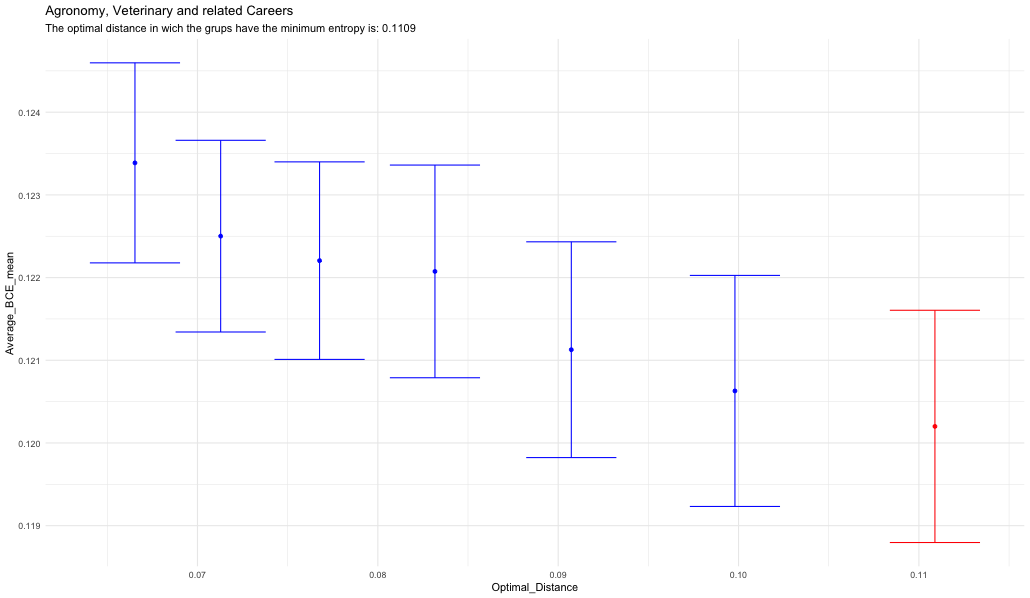
\includegraphics[width=0.8\textwidth]{Graph/Results/optimal_distance_bs30_AGRONOMY_VETERINARY_RELATED.png}
    \caption{Optimal Distance for Agronomy and Veterinary Related Majors}
    \label{fig:optimal_distance_agronomy_vet}
\end{figure}

\textbf{2. Economics and Business Related Majors}:
   Figure \ref{fig:optimal_distance_econ_bus} illustrates that the optimal distance for minimizing entropy in schooling decisions related to Economics and Business majors is 0.0832.

\begin{figure}[H]
    \centering
    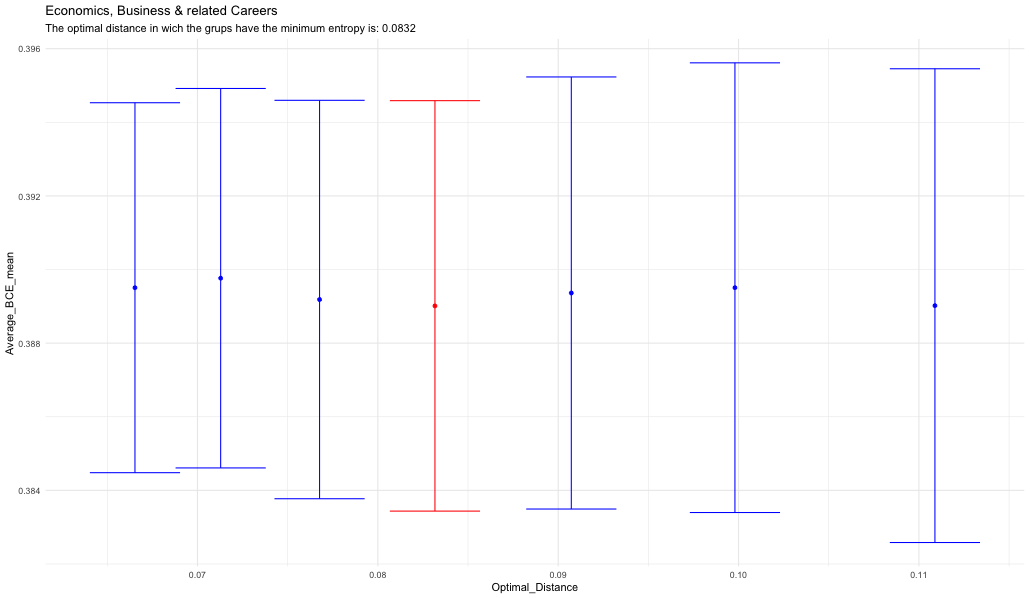
\includegraphics[width=0.8\textwidth]{Graph/Results/optimal_distance_bs30_ECONOMICS_BUSINESS_RELATED.png}
    \caption{Optimal Distance for Economics and Business Related Majors}
    \label{fig:optimal_distance_econ_bus}
\end{figure}

\textbf{ 3. Education Sciences Majors}:
   Examining Figure \ref{fig:optimal_distance_edu_sci}, we find that the optimal distance for Education Sciences majors, which minimizes entropy in schooling decisions, is 0.1109.

\begin{figure}[H]
    \centering
    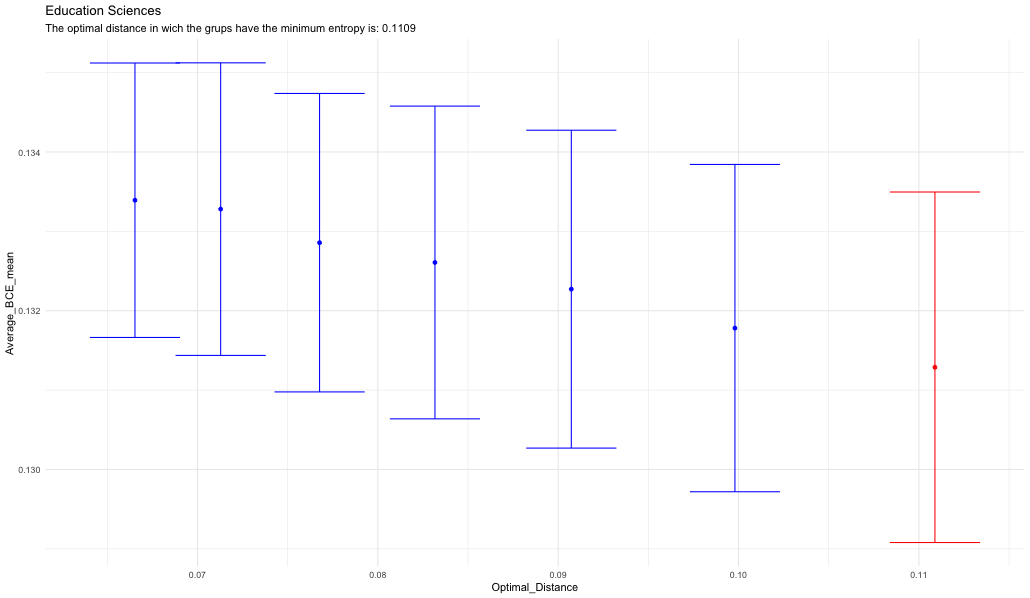
\includegraphics[width=0.8\textwidth]{Graph/Results/optimal_distance_bs30_EDUCATION_SCIENCES.png}
    \caption{Optimal Distance for Education Sciences Majors}
    \label{fig:optimal_distance_edu_sci}
\end{figure}

\textbf{ 4. Engineering and Architecture Related Majors}:
   Figure \ref{fig:optimal_distance_eng_arch} presents the optimal distance of 0.1109 for minimizing entropy in schooling decisions concerning Engineering and Architecture Related Majors.

\begin{figure}[H]
    \centering
    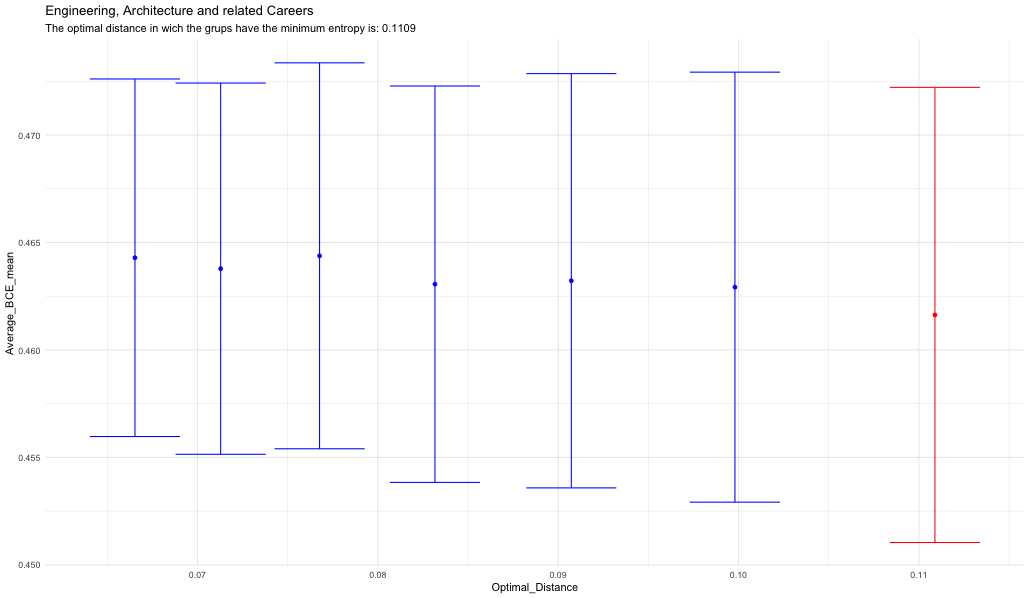
\includegraphics[width=0.8\textwidth]{Graph/Results/optimal_distance_bs30_ENG_ARCH_RELATED.png}
    \caption{Optimal Distance for Engineering and Architecture Related Majors}
    \label{fig:optimal_distance_eng_arch}
\end{figure}

\textbf{5. Fine Arts Majors}:
   In Figure \ref{fig:optimal_distance_fine_arts}, we observe that the optimal distance for minimizing entropy in schooling decisions pertaining to Fine Arts majors is 0.1109.

\begin{figure}[htbp]
    \centering
    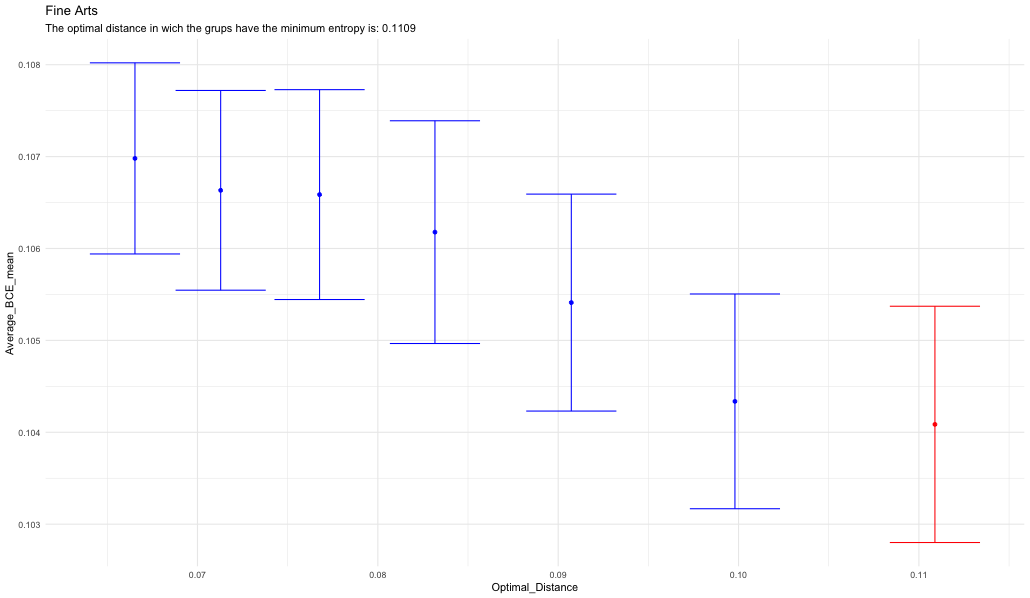
\includegraphics[width=0.8\textwidth]{Graph/Results/optimal_distance_bs30_FINE_ARTS.png}
    \caption{Optimal Distance for Fine Arts Majors}
    \label{fig:optimal_distance_fine_arts}
\end{figure}

\textbf{ 6. Health Sciences Majors}:
   The optimal distance of 0.0832, as shown in Figure \ref{fig:optimal_distance_health_sci}, minimizes entropy in schooling decisions regarding Health Sciences majors.

\begin{figure}[H]
    \centering
    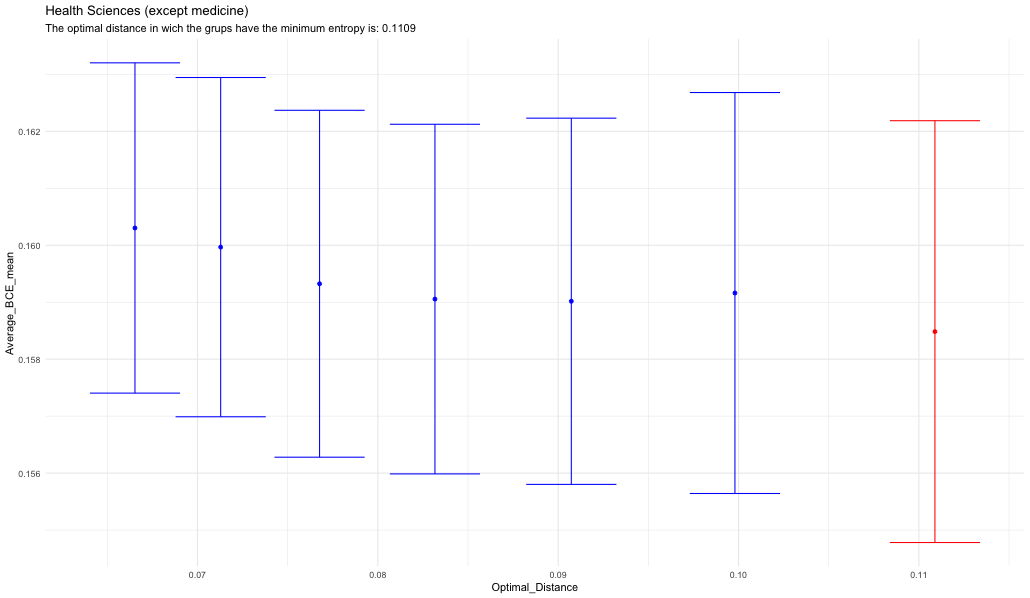
\includegraphics[width=0.8\textwidth]{Graph/Results/optimal_distance_bs30_HEALTH_SCIENCES.png}
    \caption{Optimal Distance for Health Sciences Majors}
    \label{fig:optimal_distance_health_sci}
\end{figure}

\textbf{7. Law Majors}:
   Figure \ref{fig:optimal_distance_law} illustrates that the optimal distance for minimizing entropy in schooling decisions regarding Law majors is 0.0998.

\begin{figure}[H]
    \centering
    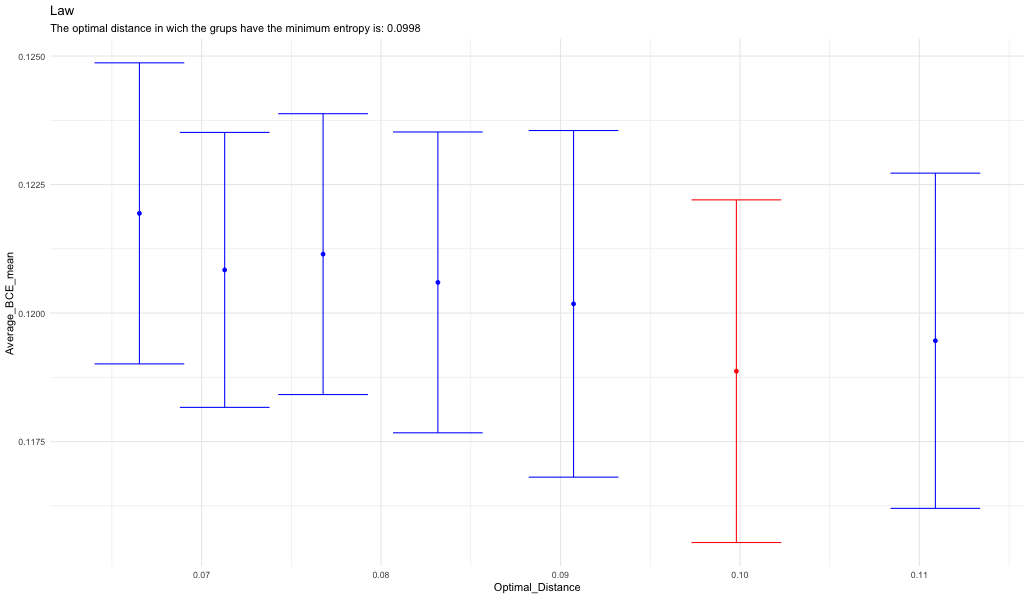
\includegraphics[width=0.8\textwidth]{Graph/Results/optimal_distance_bs30_LAW.png}
    \caption{Optimal Distance for Law Majors}
    \label{fig:optimal_distance_law}
\end{figure}

\textbf{8. Mathematics and Natural Sciences Majors}:
   Examining Figure \ref{fig:optimal_distance_math_natural_sci}, we find that the optimal distance for Mathematics and Natural Sciences majors, which minimizes entropy in schooling decisions, is 0.1109.

\begin{figure}[H]
    \centering
    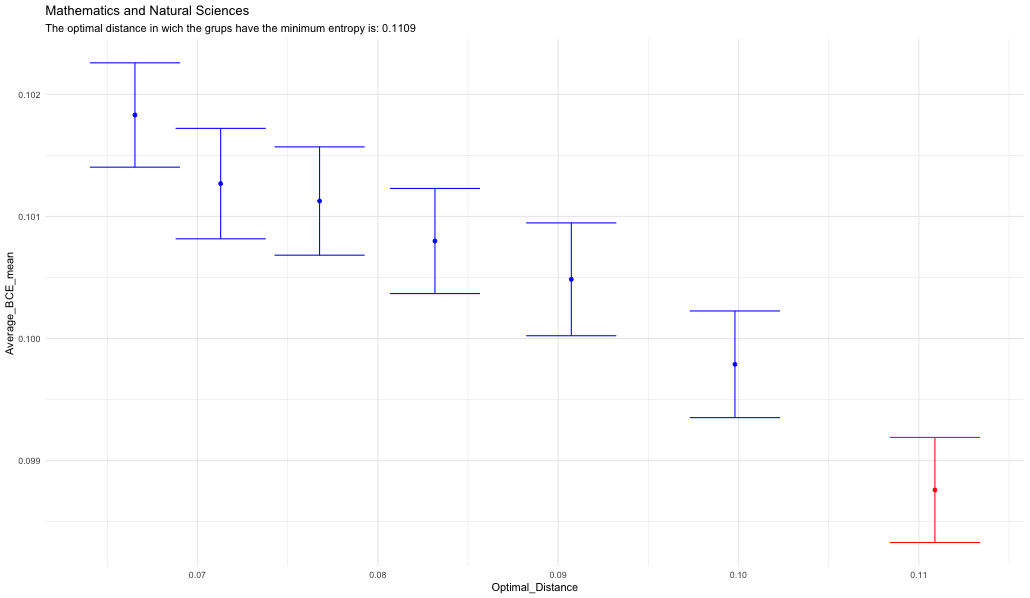
\includegraphics[width=0.8\textwidth]{Graph/Results/optimal_distance_bs30_MATHEMATICS_NATURAL_SCIENCES.png}
    \caption{Optimal Distance for Mathematics and Natural Sciences Majors}
    \label{fig:optimal_distance_math_natural_sci}
\end{figure}

\textbf{ 9. Medicine Majors}:
   As depicted in Figure \ref{fig:optimal_distance_medicine}, the optimal distance that minimizes the entropy in schooling decisions regarding the selection of Medicine majors is 0.1109.

\begin{figure}[htbp]
    \centering
    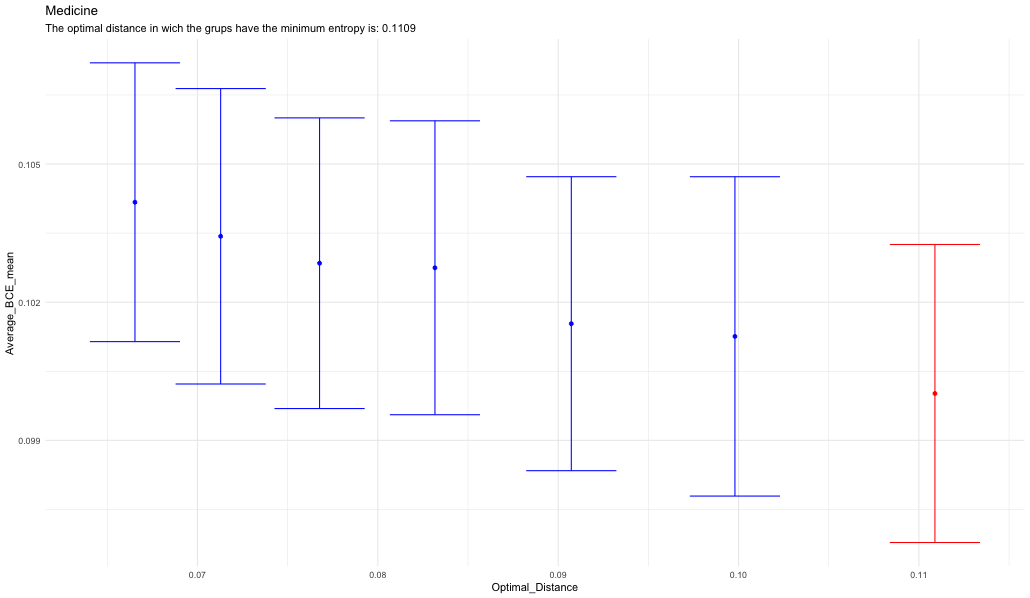
\includegraphics[width=0.8\textwidth]{Graph/Results/optimal_distance_bs30_MEDICINE.png}
    \caption{Optimal Distance for Medicine Majors}
    \label{fig:optimal_distance_medicine}
\end{figure}

\textbf{ 10. No Studies}:
    Figure \ref{fig:optimal_distance_no_studies} presents the optimal distance of 0.0832 for minimizing entropy in schooling decisions concerning not pursuing further studies.

\begin{figure}[H]
    \centering
    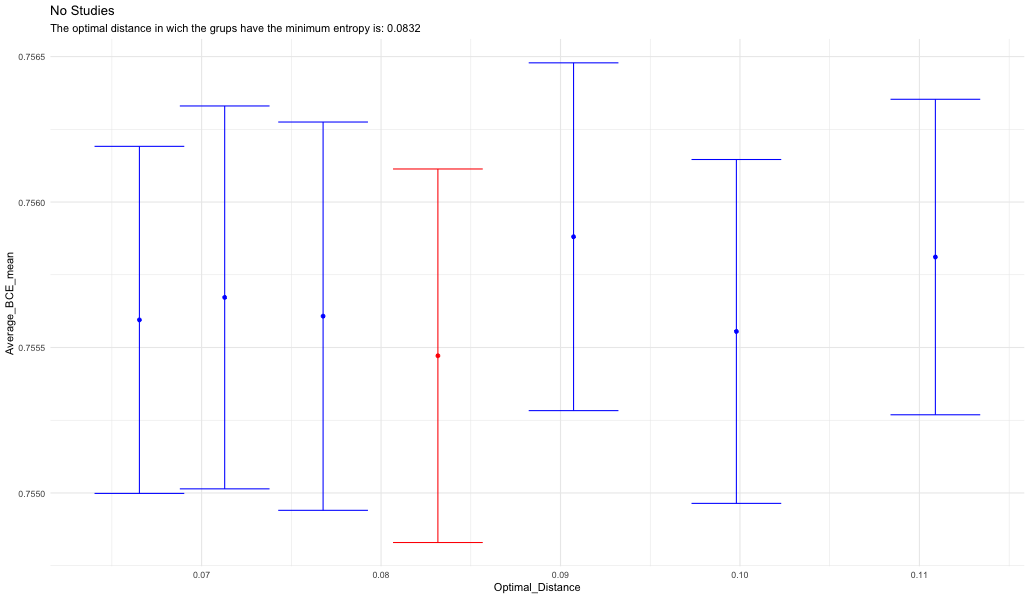
\includegraphics[width=0.8\textwidth]{Graph/Results/optimal_distance_bs30_NO_STUDIES.png}
    \caption{Optimal Distance for Not Pursuing Further Studies}
    \label{fig:optimal_distance_no_studies}
\end{figure}

\textbf{ 11. Social Sciences and Humanities Majors}:
    The optimal distance of 0.1109, as shown in Figure \ref{fig:optimal_distance_soc_sci_hum}, minimizes entropy in schooling decisions regarding Social Sciences and Humanities majors.

\begin{figure}[H]
    \centering
    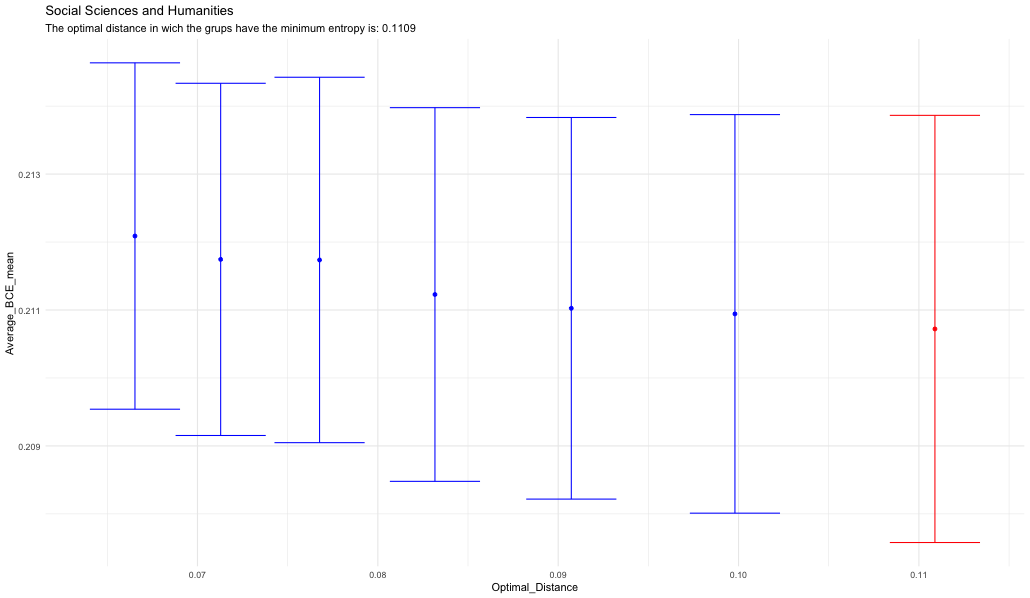
\includegraphics[width=0.8\textwidth]{Graph/Results/optimal_distance_bs30_SOCIAL_SCIENCES_HUMANITIES.png}
    \caption{Optimal Distance for Social Sciences and Humanities Majors}
    \label{fig:optimal_distance_soc_sci_hum}
\end{figure}
\label{section:app}
\end{document}




 
